%!TEX program = xelatex*2
%!TEX root = elegantnote.tex
% \documentclass[cn,blue,14pt,screen]{elegantnote}
% pad、pc、kindle、normal、screen
\documentclass[cn,blue,12pt,normal]{elegantnote}
\title{数值最优化算法及应用}
\author{\href{mailto:zhangxinhang19@foxmail.com}{张鑫航}\\
23010050}
\institute{国防科技大学}
\version{1.0}
\date{\zhtoday}

\usepackage{array}
\usepackage{bigstrut}
\usepackage{float}
\usepackage{multirow}
\usepackage{wrapfig}
\usepackage{colortbl}
\usepackage{cancel}
\usepackage{mathtools}
%green color
\definecolor{main1}{RGB}{210,168,75}
\definecolor{seco1}{RGB}{9,80,3}
\definecolor{thid1}{RGB}{0,175,152}
%cyan color
\definecolor{main2}{RGB}{239,126,30}
\definecolor{seco2}{RGB}{0,175,152}
\definecolor{thid2}{RGB}{236,74,53}
%cyan color
\definecolor{main3}{RGB}{127,191,51}
\definecolor{seco3}{RGB}{0,145,215}
\definecolor{thid3}{RGB}{180,27,131}

% ---自定义命令--- %
% 星号
\usepackage{tikz}
\usetikzlibrary{shapes.geometric}
\newcommand{\Stars}[2][fill=yellow,draw=orange]{\begin{tikzpicture}[baseline=-0.35em,#1]
\foreach \X in {1,...,5}
{\pgfmathsetmacro{\xfill}{min(1,max(1+#2-\X,0))}
\path (\X*1.1em,0) 
node[star,draw,star point height=0.25em,minimum size=1em,inner sep=0pt,
path picture={\fill (path picture bounding box.south west) 
rectangle  ([xshift=\xfill*1em]path picture bounding box.north west);}]{};
}
\end{tikzpicture}}

\begin{document}
\maketitle
\centerline{
  
\includegraphics[width=0.2\textwidth]{figure/logo.pdf}
}
使用\textcolor{cyan}{\LaTeX{}}生成。
\newpage
\tableofcontents
\newpage

\section{无约束优化}
\subsection{最优性条件的应用}
\begin{theorem}
    设$\boldsymbol{x}^*$为优化问题$\min\limits_x\in\mathbb{R}^nf(\boldsymbol{x})$ 的最优解,则 $\nabla f(\boldsymbol{x}^*)=\mathbf{0},\nabla^2f(\boldsymbol{x}^*)$半正定。
\end{theorem}
\begin{theorem}
    对优化问题$\min\limits_{\boldsymbol{x}\in\mathbb{R}^n}f(\boldsymbol{x})$ ,设$\nabla f(\boldsymbol{x}^*)=0,\nabla^2f(\boldsymbol{x}^*)$正定,
则$\boldsymbol{x}^*$是该优化问题的严格最优解,
\end{theorem}
\begin{example}
    优化问题的解析解\Stars{5}
    \[
        \min\limits_{x>0,y\geqslant 0}f(x,y)=\dfrac{10}{x}+\dfrac{(x-y)^{2}}{2x}+\dfrac{3y^{2}}{2x}
    \]
    \begin{solution}
        先忽略约束:利用$\min\limits_{x,y}f(x,y)=\min\limits_x\min\limits_yf(x,y)$,先固定$x$,关于$y$做内层优化,再求解关于$x$的外层优化
        \[
            \min\limits_{y}f(x,y)=\frac{10}{x}+\frac{(x-y)^{2}}{2x}+\frac{3y^{2}}{2x}
        \]
        目标函数关于$y$为凸函数,利用最优性条件得最优解
        \[
            \begin{array}{c}
                f(x,y)=\dfrac{1}{2x}\left( 20+x^2-2xy+4y^2 \right)\\
                y = \dfrac{1}{4}x
            \end{array}
        \]
        将上述最优解代入目标函数得外层优化问题
        \[
            \min f(x)=\dfrac{10}{x}+\dfrac{3}{8}x
        \]
        目标函数关于$x$为凸函数(二阶导数大于0)。再利用最优性条件得$x=\dfrac43\sqrt{15},y=\dfrac{1}{4}x=\dfrac{1}{3}\sqrt{15}$

        它们满足约束条件,自然为原问题的最优解。
    \end{solution}
\end{example}
\subsection{最速下降算法}
\begin{example}
    利用最速下降方法求\Stars{5}
    \[
        \min\limits_{\boldsymbol{x}\in\mathbb{R}^2}f(x_1,x_2) = \dfrac{1}{3}x_{1}^2+\dfrac{1}{2}x_2^2
    \]
    \begin{solution}
        显然,唯一最优解$\boldsymbol{x}^* = \left( 0,0 \right)$,取初始点$\boldsymbol{x}_0 = (3,2)$,那么最速下降方法产生的迭代点列
        $\boldsymbol{x}_k$

        \begin{itemize}
            \item $k = 0$时
            \[
                \boldsymbol{g}_0 = \nabla f(\boldsymbol{x}^{(0)})  =  \begin{pmatrix}
                    2\\2
                \end{pmatrix}
            \]
            \[
                \begin{aligned}
                    \alpha_0 &= \arg\min_{\alpha>0}f(\boldsymbol{x}^{(0)}-\alpha\boldsymbol{g}^{(0)})\\
                    &=\arg\min_{\alpha>0}\dfrac{1}{3}\left( 10\alpha^2-24\alpha+\cdots \right) = \dfrac{6}{5}
                \end{aligned}
            \]
            \[
                \boldsymbol{x}^{(1)} = \boldsymbol{x}^{(0)}-\alpha\boldsymbol{g}^{(0)  } = (3,2)-\dfrac{6}{5}(2,2)  = (\dfrac{3}{5},-\dfrac{2}{5})
            \]
            \item $k = 1,\cdots $
        \end{itemize}
        综上,得到迭代序列$\boldsymbol{x}^{(k)}$
        \[
            \boldsymbol{x}_{k}=\left(\frac{3}{5^{k}};(-1)^{k}\frac{2}{5^{k}}\right)\overset{k\to\infty}{\longrightarrow}(0;0)
        \]
        全局收敛,收敛速度线性!
        有$\|\boldsymbol{x}_k-\boldsymbol{x}^*\|=\sqrt{13}\big(\frac15\big)^k.$那么
        \[
            \begin{aligned}
                \frac{\|\boldsymbol{x}_{k+1}-\boldsymbol{x}^*\|}{\|\boldsymbol{x}_k-\boldsymbol{x}^*\|} & =\frac15<\frac15\sqrt{\frac32}=\frac{\lambda_1-\lambda_2}{\lambda_1+\lambda_2}\sqrt{\frac{\lambda_1}{\lambda_2}}\\
                \frac{f(\boldsymbol{x}_{k+1})-f(\boldsymbol{x}^*)}{f(\boldsymbol{x}_k)-f(\boldsymbol{x}^*)} & =\frac1{25}=\left(\frac{\lambda_1-\lambda_2}{\lambda_1+\lambda_2}\right)^2
            \end{aligned}
        \]
    \end{solution}
\end{example}
\subsection{牛顿算法}
\begin{example}
    用牛顿法求解\Stars{5}
    \[
        \min f(x)=\sqrt{1+x^2}
    \]
    \begin{solution}
        $0$为最优解
    
        目标函数导数$f'(x)=\dfrac{x}{\sqrt{1+x^2}}\quad f''(x)=\dfrac{1}{(1+x^2)^{3/2}}$
        
        迭代过程
        \[
            \begin{aligned}
                x_{k+1}& =x_{k}-\frac{f'(x_{k})}{f''(x_{k})}  \\
                &=x_{k}-x_{k}(1+x_{k}^{2}) \\
                &=-x_{k}^{3}
            \end{aligned}
        \]
        \begin{itemize}
            \item 当$x_0<1$,算法快速收敛到最优解;
            \item 当$x_0\geqslant 1$,算法不收敛
        \end{itemize}
    \end{solution}
\end{example}

\begin{example}
    用牛顿算法求解\Stars{5}{}
    \[
        \min f(\boldsymbol{x}) = 4x_1^2+x_2^2-x_1^2x_2
    \]
    \begin{solution}
        最优解$\boldsymbol{x}^* = (0,0)$

        函数鞍$(2\sqrt{2},4),\,(-2\sqrt{2},4)$

        目标函数梯度信息
        \[
            \nabla f(\boldsymbol{x}) = \begin{pmatrix}
                8x_1-2x_1x_2\\2x_2-x_1^2
            \end{pmatrix},\quad
            \nabla^2 f(\boldsymbol{x}) = \begin{pmatrix}
                8-2x_2 & -2x_1 \\
                -2-x_1 & 2 
            \end{pmatrix},
        \]
        取精度$\varepsilon = 10^{-3}$和不同初始点
    \end{solution}
\end{example}
\subsection{线性共轭梯度法}
\begin{example}
    利用共轭梯度法求$\boldsymbol{Ax} = \boldsymbol{b} = \boldsymbol{0}$或者说,利用共轭梯度法求\quad\Stars{5}
    \[
        \min x_1^2+\dfrac{1}{2}x_2^2+\dfrac{1}{2}x_3^2
    \]
    其中,
    \[
        \boldsymbol{A} = \begin{bmatrix}
            1 & 0 & 0\\
            0 & \frac{1}{2} & 0 \\
            0 & 0 & \frac{1}{2}
        \end{bmatrix},\quad
        \boldsymbol{b} = \begin{pmatrix}
            0\\0\\0
        \end{pmatrix}
    \]

    \begin{solution}
        取初始点$\boldsymbol{x}_0 = (1,1,1)^{\mathrm{T}} $,迭代过程:
        \begin{enumerate}
            \item $\boldsymbol{x}_0 = (1,1,1)^{\mathrm{T}} $,$\boldsymbol{g}_0 = \boldsymbol{Ax}_0-\boldsymbol{0} = (2,1,1)^{\mathrm{T}}$,$\beta_{-1} = 0$,$\boldsymbol{d}_{0} = -\boldsymbol{g}_0$.
            \[
                \begin{array}{ll}
                    \alpha &= \arg\min f(\boldsymbol{x}_0+\alpha \boldsymbol{d}_0)\\
                    & = (1-2\alpha)^2+\frac{1}{2}(1-\alpha)^2+\frac{1}{2}(1-\alpha)^2 = \frac{3}{5}
                \end{array}
            \]
            \item $\boldsymbol{x}_1 = \boldsymbol{x}_0+\alpha_0\boldsymbol{d}_0=\frac{1}{5}(-1,2,2)^{\mathrm{T}} $,$\boldsymbol{g}_1 = \boldsymbol{Ax}_1-\boldsymbol{0} = \frac{1}{5}(-1,2,2)^{\mathrm{T}}$,$\beta_{0} = \frac{\boldsymbol{g}_1^{\mathrm{T}}\boldsymbol{g}_1}{\boldsymbol{g}_0^{\mathrm{T}}\boldsymbol{g}_0}= \frac{2}{25}$ 
            \[
                \boldsymbol{d}_{1} = -\boldsymbol{g}_1+\beta_{0}\boldsymbol{d}_0 = -\frac{6}{25}(1,-2,-2)^{\mathrm{T}}
            \]
            \[
                \begin{array}{ll}
                    \alpha &= \arg\min f(\boldsymbol{x}_0+\alpha \boldsymbol{d}_0)\\
                    & = (1-2\alpha)^2+\frac{1}{2}(1-\alpha)^2+\frac{1}{2}(1-\alpha)^2 = \frac{3}{5}
                \end{array}
            \]
            \item $\boldsymbol{x}_2 = \boldsymbol{x}_1 + \alpha_1\boldsymbol{d}_1 = \boldsymbol{0}$,$\|\boldsymbol{g}_2\| = 0$,终止。
        \end{enumerate}

        \begin{table}[htbp]
            \centering
            \begin{tabular}{c|c|c|c|c|c}
                \hline
                $k$ & $\boldsymbol{x}_k$ & $\boldsymbol{g}_k$ & $\beta_{k-1}$ & $\boldsymbol{d}_k$ & $\alpha_k$\\\hline
                $0$ & $ (1,1,1)^{\mathrm{T}} $ & $(2,1,1)^{\mathrm{T}}$ & $0$ & $ -(2,1,1)^{\mathrm{T}} $ & $\frac{3}{5}$\\\hline
                $1$ & $ \frac{1}{5}(-1,2,2)^{\mathrm{T}} $ & $\frac{1}{5}(-2,2,2)^{\mathrm{T}}$ & $\frac{2}{25}$ & $ -\frac{6}{25}(1,-2,-2)^{\mathrm{T}} $ & $\frac{5}{6}$\\\hline
                $2$ & $(0,0,0)^{\mathrm{T}}$ & $(0,0,0)^{\mathrm{T}}$ & \\\hline
            \end{tabular}
        \end{table}
    \end{solution}
\end{example}

\section{无约束优化最优性问题}
\subsection{无约束优化最优性条件}

数学模型$\min\limits_{\boldsymbol{x}\in\mathbb{R}^n}f(\boldsymbol{x})$,其中$f:\mathbb{R}^n\to \mathbb{R}$

\begin{note}
    最优解判定:
    \begin{itemize}
        \item 直观地,验证最优解,需将其和附近点的目标函数值逐一比较,工作量太大。
        \item 利用目标函数的连续可微性质,可建立一个简易的判断方法, 这就是光滑优化问题的最优性条件.
    \end{itemize}
\end{note}

\begin{theorem}[无约束优化问题]
    $\boldsymbol{x}^*$是$\min\limits_{\boldsymbol{x}\in\mathbb{R}^n}f(\boldsymbol{x})$(局部)最优解,则$\nabla f(\boldsymbol{x}^*) = \boldsymbol{0}$
\end{theorem}
\begin{proof}
    反证法。取$\boldsymbol{d} = -\nabla f(\boldsymbol{x}^*)$,$\alpha>0$充分小。则
    \[
        \begin{array}{ll}
            f(\boldsymbol{x}^*+\alpha\boldsymbol{d})&=f(\boldsymbol{x}^*)+\alpha\nabla f(\boldsymbol{x}^*)^\mathrm{T}\boldsymbol{d}+o(\alpha)\\
            &=f(\boldsymbol{x}^*)-\alpha\|\nabla f(\boldsymbol{x}^*)\|^2+o(\alpha)\\
            &<f(\boldsymbol{x}^*)
        \end{array}
    \]
    和$\boldsymbol{x}^*$是$\min\limits_{\boldsymbol{x}\in\mathbb{R}^n}f(\boldsymbol{x})$(局部)最优解矛盾。证毕!
\end{proof}
\begin{definition}[凸函数]
    $f\left(\lambda\boldsymbol{x}+(1-\lambda)\boldsymbol{y}\right)\leqslant\lambda f(\boldsymbol{x})+(1-\lambda)f(\boldsymbol{y}),\forall\boldsymbol{x},\boldsymbol{y}\in\mathbb{R}^n,\lambda\in[0,1]$或者$f\left(\sum\limits_{i=1}^m\lambda_i\boldsymbol{x}_i\right)\leqslant\sum\limits_{i=1}^m\lambda_if(\boldsymbol{x}_i),\forall \boldsymbol{x}_i\in\mathbb{R}^n,\lambda_i\geqslant 0,i=1,2,\cdots,m,\sum\limits_{i=1}^m\lambda_i=1$
\end{definition}
\begin{definition}[凸组合]
    设$\boldsymbol{x}_1,\boldsymbol{x}_2,\cdots ,\boldsymbol{x}_m\in\mathbb{R}^n$,$\lambda_{1}+\lambda_{2}+\cdots+\lambda_{m}=1,\lambda_{1},\lambda_{2},\cdots,\lambda_{m}\in (0,1)$,则称$\lambda_1\boldsymbol{x}_1+\lambda_2\boldsymbol{x}_2+\cdots+\lambda_m\boldsymbol{x}_m$为$\boldsymbol{x}_1,\boldsymbol{x}_2,\cdots ,\boldsymbol{x}_m$的一个凸组合。
\end{definition}
\begin{definition}[凸函数的等价定义1(上图)]
    函数$f$的上图$\operatorname{epi}(f)$是凸集。$\operatorname{epi}(f):=\{(\boldsymbol{x},\alpha)\in\mathbb{R}^n\times\mathbb{R}\mid\alpha\geqslant f(\boldsymbol{x})\}$是凸集。
    \begin{figure}[H]
        \centering
        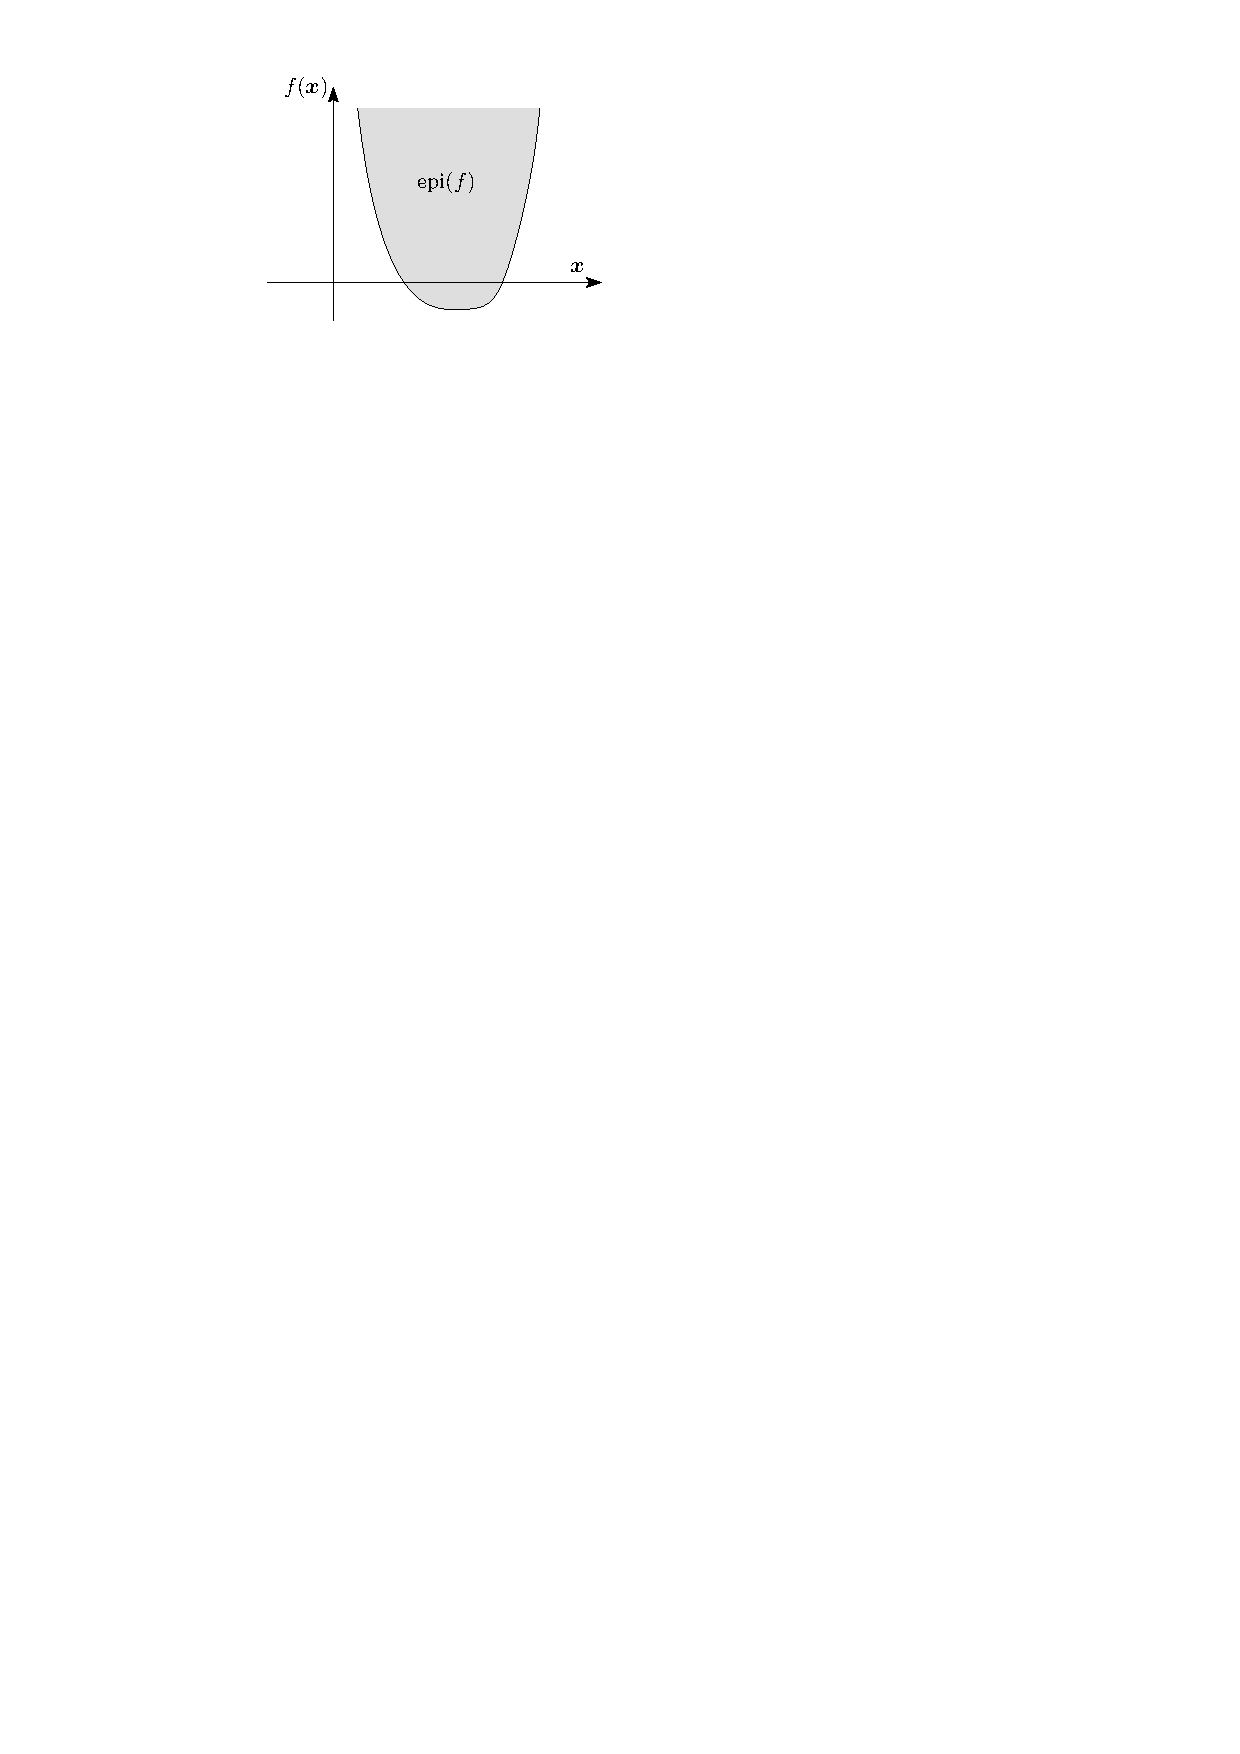
\includegraphics{image/epi.pdf}
    \end{figure}
\end{definition}
\begin{definition}[凸函数的等价定义2(连续可微)]
    切平面在曲面下方。
    $f(\boldsymbol{y})-f(\boldsymbol{x})\geqslant\nabla f(\boldsymbol{x})^{\mathrm{T}}(\boldsymbol{y}-\boldsymbol{x}),\forall \boldsymbol{x},\boldsymbol{y}\in\mathbb{R}^{n}$
\end{definition}
\begin{definition}[凸函数的等价定义3(二阶连续可微)]
    $\boldsymbol{h}^{T}\nabla f(\boldsymbol{x})\boldsymbol{h}\geqslant 0,\forall \boldsymbol{x},\boldsymbol{h}\in \mathbb{R}^n$
\end{definition}
\begin{definition}[一致凸函数(凸函数的加强版)]
    对函数$f:\mathbb{R}^n\to \mathbb{R}$,若存在$\eta>0$,使对任意$\boldsymbol{x},\boldsymbol{y}\in \mathbb{R}$和$\lambda\in (0,1)$成立
    \[
        f(\lambda\boldsymbol{x}+(1-\lambda)\boldsymbol{y})\leqslant\lambda f(\boldsymbol{x})+(1-\lambda)f(\boldsymbol{y})-\lambda(1-\lambda)\eta\|\boldsymbol{x}-\boldsymbol{y}\|^2
    \]
    则称其为一致凸函数,又称强凸函数。
    \begin{figure}[H]
        \centering
        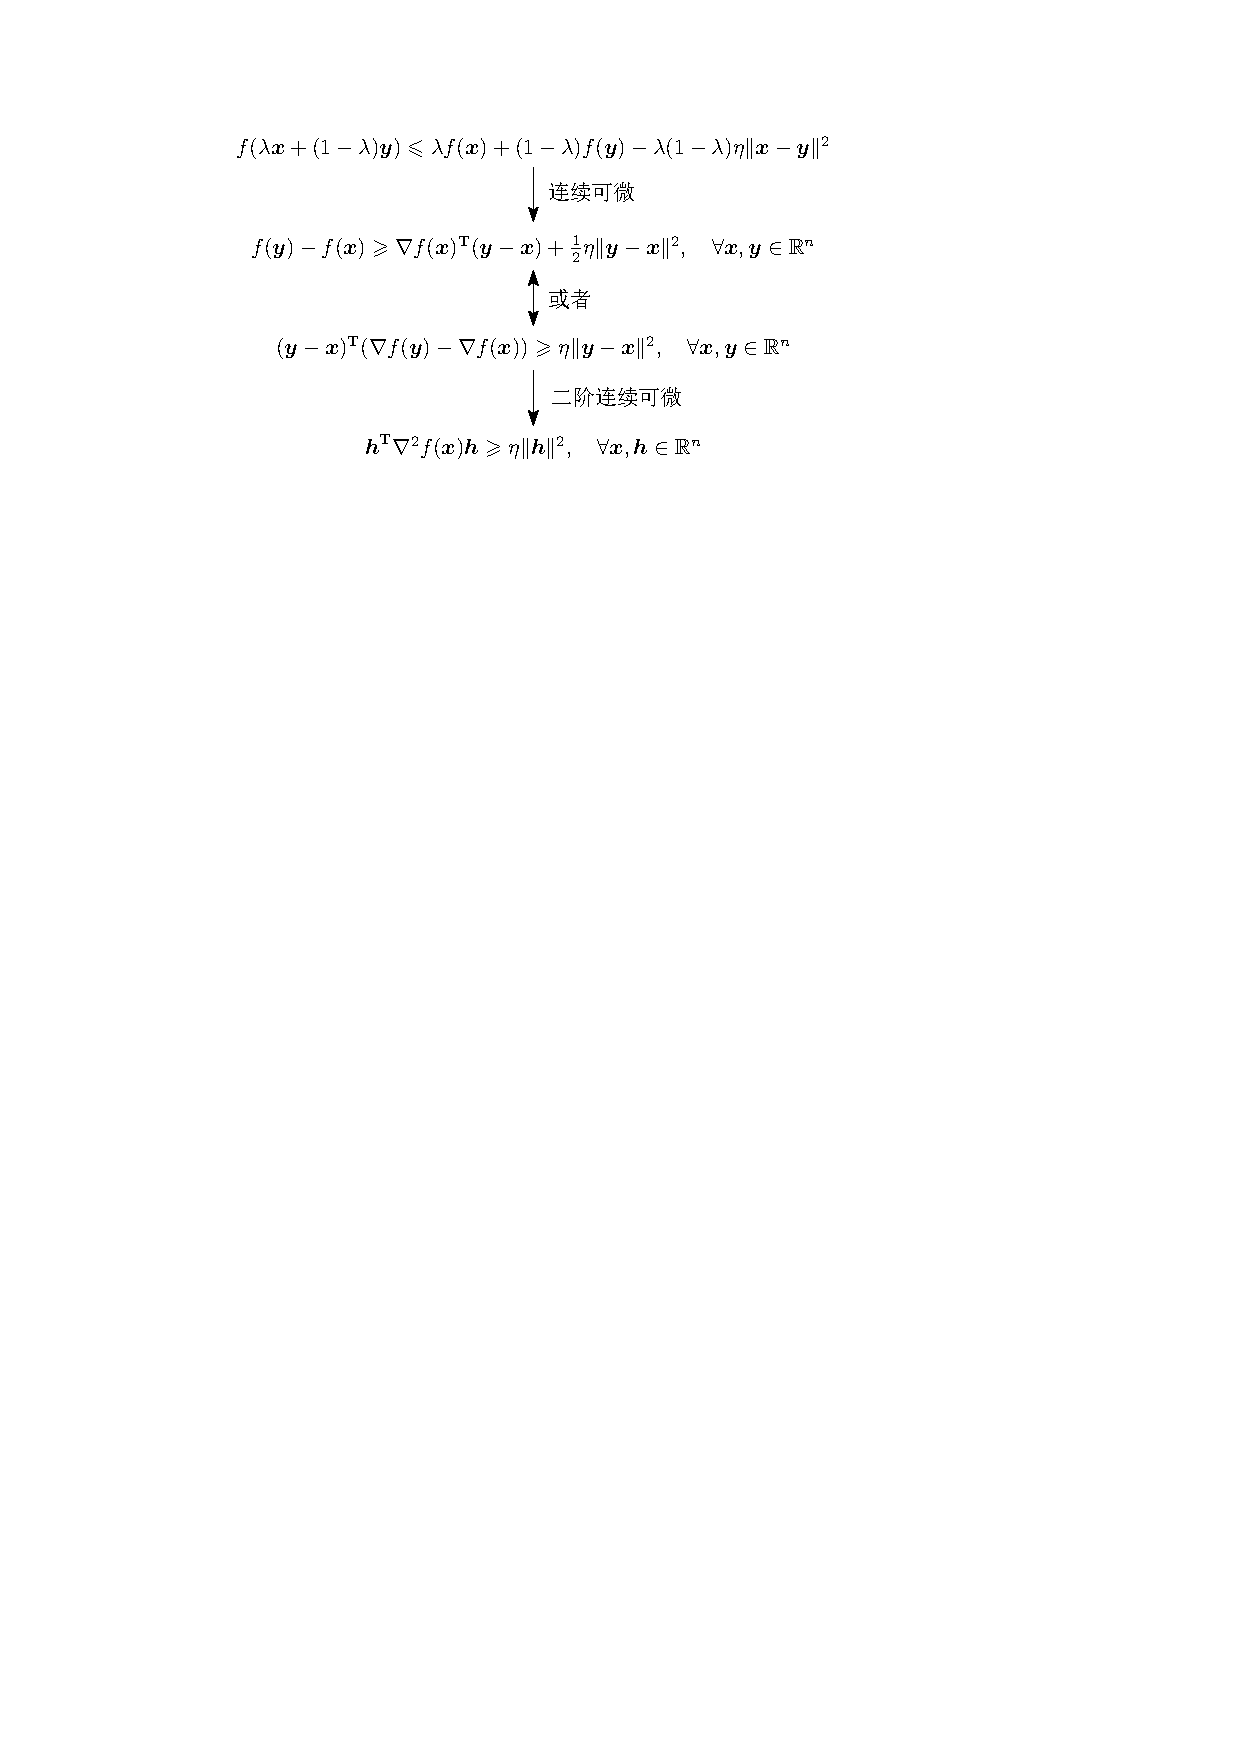
\includegraphics{image/一致凸函数.pdf}
    \end{figure}
\end{definition}
\begin{note}
    线性函数是凸函数但不一致凸。对二次函数,一致凸与严格凸等价。
\end{note}
\begin{note}
    $f(\boldsymbol{x})$一致凸等价于$f(\boldsymbol{x})-\eta \|\boldsymbol{x}\|^2$为凸函数,存在$\eta>0$
\end{note}
\begin{theorem}[凸优化]
    $\min\limits_{\boldsymbol{x}\in\mathbb{R}^n}f(\boldsymbol{x})$,$f:\mathbb{R}^n\to \mathbb{R}$为连续可微的凸函数。凸优化问题的稳定点为其全局最优解。
\end{theorem}
\begin{proof}
    利用凸函数的性质
    \[
        \begin{array}{c}
            f(\boldsymbol{x})-f(\boldsymbol{x}^*)\geqslant \left<\nabla f(\boldsymbol{x}^*),\boldsymbol{x}-\boldsymbol{x}^*\right> = 0\\
            f(\boldsymbol{x})>f(\boldsymbol{x}^*)
        \end{array}
    \]
\end{proof}
\begin{theorem}[无约束优化二阶最优性条件]
    设$\boldsymbol{x}^*$为优化问题$\min\limits_{\boldsymbol{x}\in\
    \mathbb{R}^n}f(\boldsymbol{x})$的最优解,则$\nabla f(\boldsymbol{x}^*) = \boldsymbol{0},\nabla^2f(\boldsymbol{x}^*)$半正定。
\end{theorem}
\begin{proof}
    结论$\nabla f(\boldsymbol{x}^{*})=\mathbf{0}$已证。
    
    反设$\nabla^2 f(\boldsymbol{x}^{*})$非半正定,则存在向量$\boldsymbol{d}$使得
    \[
        \boldsymbol{d}^\mathrm{T}\nabla^2f(\boldsymbol{x^*})\boldsymbol{d}<0.
    \]
    取$\alpha>0$充分小。由泰勒展开式
    \[
        \begin{array}{ll}
            f(\boldsymbol{x}^{*}+\alpha\boldsymbol{d})& =f(\boldsymbol{x}^{*})+\alpha\nabla f(\boldsymbol{x}^{*})^{\mathrm{T}}\boldsymbol{d}+\frac{1}{2}\alpha^{2}\boldsymbol{d}^{\mathrm{T}}\nabla^{2}f(\boldsymbol{x}^{*})\boldsymbol{d}+o(\alpha^{2})  \\
            &<f(\boldsymbol{x}^{*}).
        \end{array}
    \]
    得矛盾。证毕!
\end{proof}
\begin{note}
    二阶必要条件的非充分性:
    
    函数$f(x)$在零点满足$\nabla f(\boldsymbol{x}^*) = \boldsymbol{0}$,$\nabla^2f(\boldsymbol{x})$半正定,但但零点不是其最优值点。
\end{note}
\begin{theorem}[二阶充分条件]
    对优化问题$\min\limits_{\boldsymbol{x}\in \mathbb{R}^n}f(\boldsymbol{x})$,设$\nabla f(\boldsymbol{x}) = \boldsymbol{0}$,$\nabla^2\boldsymbol{f(\boldsymbol{x}^*)}$正定,则$\boldsymbol{x}^*$为该优化问题的严格最优解
\end{theorem}
\begin{proof}
    对任意充分靠近$\boldsymbol{x}^*$的$\boldsymbol{x}$,存在单位向量$\boldsymbol{d}$,使得
    \[
        \boldsymbol{x} = \boldsymbol{x}^*+\alpha\boldsymbol{d}   
    \]
    其中$\alpha>0$充分小。则
    \[
        f(\boldsymbol{x})=f(\boldsymbol{x}^{*})+\frac{1}{2}\alpha^{2}\boldsymbol{d}^{\mathrm{T}}\nabla^{2}f(\boldsymbol{x}^{*})\boldsymbol{d}+o(\alpha^{2})>f(\boldsymbol{x}^{*}).
    \]
\end{proof}
\begin{example}
    $\min\limits_{x>0,y\geqslant 0}f(x,y)=\dfrac{10}{x}+\dfrac{(x-y)^{2}}{2x}+\dfrac{3y^{2}}{2x}$\quad \Stars{5}

    先忽略约束:利用$\min\limits_{x,y}f(x,y)=\min\limits_x\min\limits_yf(x,y)$,先固定$x$,关于$y$做内层优化,再求解关于$x$的外层优化
    \[
        \min\limits_{y}f(x,y)=\frac{10}{x}+\frac{(x-y)^{2}}{2x}+\frac{3y^{2}}{2x}
    \]
    目标函数关于$y$为凸函数,利用最优性条件得最优解
    \[
        \begin{array}{c}
            f(x,y)=\dfrac{1}{2x}\left( 20+x^2-2xy+4y^2 \right)\\
            y = \dfrac{1}{4}x
        \end{array}
    \]
    将上述最优解代入目标函数得外层优化问题
    \[
        \min f(x)=\dfrac{10}{x}+\dfrac{3}{8}x
    \]
    目标函数关于$x$为凸函数(二阶导数大于0)。再利用最优性条件得$x=\frac43\sqrt{15},y=\frac{1}{4}x=\frac{1}{3}\sqrt{15}$

    它们满足约束条件,自然为原问题的最优解。
\end{example}

\subsection{无约束优化线搜索方法}
\subsubsection{精确线搜索方法}
\begin{note}
    优化模型:
    \[
        \min\limits_{\boldsymbol{x}\in\mathbb{R}^n}f(\boldsymbol{x})
    \]
    其中,$f:\mathbb{R}^n\to\mathbb{R}$连续可微。
\end{note}
\begin{note}
    有关记号:
    \[
        \begin{array}{ll}
            \boldsymbol{g}_k=\nabla f(\boldsymbol{x}_k), & \boldsymbol{g}(\boldsymbol{x})=\nabla f(\boldsymbol{x})\\
            \boldsymbol{G}_k=\nabla^2f(\boldsymbol{x}_k), & \boldsymbol{G}(\boldsymbol{x})=\nabla^2f(\boldsymbol{x}).
        \end{array}
    \]
\end{note}
我们先回顾作为最速下降方向的负梯度方向。假设$\nabla f(\boldsymbol{x})\neq \boldsymbol{0}$。固定方向$\boldsymbol{d}\in \mathbb{R}^n$且$\|\boldsymbol{d}\| = 1$。考虑沿此方向函数值的变化。由可微的定义可知
\[
    f(\boldsymbol{x}+\tau \boldsymbol{d}) = f(\boldsymbol{x}) + \tau \nabla f(\boldsymbol{x})^{\mathrm{T}}\boldsymbol{d} + o(\tau),\ \tau>0
\]
当$\nabla f(\boldsymbol{x})^{\mathrm{T}}\boldsymbol{d}<0 $时,由于$\frac{o(\tau)}{\tau}\to 0,\tau\to 0_{+}$可知,存在$\varepsilon >0$,使得当$0<\tau<\varepsilon$时,
\[
    \dfrac{o(\tau)}{\tau}\leq -\dfrac{\nabla f(\boldsymbol{x})^{\mathrm{T}}\boldsymbol{d}}{2}
\]
此时
\[
    f(\boldsymbol{x}+\tau \boldsymbol{d})-f(\boldsymbol{x})\leq \dfrac{\tau}{2}\cdot \nabla f(\boldsymbol{x})^{\mathrm{T}}\boldsymbol{d}< 0
\]
上式表明,从$\boldsymbol{x}$点沿$\boldsymbol{d}$方向出发,当步长$\tau <\varepsilon$时,
\[
    f(\boldsymbol{x}+\tau \boldsymbol{d})<f(\boldsymbol{x})
\]
因此,称满足条件$\nabla f(\boldsymbol{x})^{\mathrm{T}}\boldsymbol{d}<0$的方向为下降方向。而称下降最快或$\nabla f(\boldsymbol{x})^{\mathrm{T}}\boldsymbol{d}$最小的方向为最速下降方向,也即
\[
    \begin{array}{c}
        \hat{\boldsymbol{d}} = \arg\min \{\nabla f(\boldsymbol{x})^{\mathrm{T}}\boldsymbol{d}\}\\
        \text{s.t.} \|\boldsymbol{d}\|=1
    \end{array} 
\]
则$\boldsymbol{d} = -\frac{\nabla f(\boldsymbol{x})}{\|\nabla f(\boldsymbol{x})\|}$。事实上,有Cauchy-Schwarz不等式
\[
    |\nabla f(\boldsymbol{x})^{\mathrm{T}} \boldsymbol{d}|\leq \|\nabla f(\boldsymbol{x}) \|\cdot \|\boldsymbol{d} \|\leq \|\nabla f(\boldsymbol{x}) \|
\]
可知
\[
    -\|\nabla f(\boldsymbol{x}) \| \leq \nabla f(\boldsymbol{x})^{\mathrm{T}} \boldsymbol{d} \leq \|\nabla f(\boldsymbol{x}) \|
\]
从而$\hat{\boldsymbol{d}} = \dfrac{\nabla f(\boldsymbol{x})}{\|\nabla f(\boldsymbol{x})\|}$可取得下界$-\|\nabla f(\boldsymbol{x}) \|$。
\begin{note}
    算法分析:
    \begin{itemize}
        \item 迭代过程:$\boldsymbol{x}_{k+1} = \boldsymbol{x}_k+\alpha_k \boldsymbol{d}_k$
        \item 精确线搜索(最优步长):$\alpha = \arg\min\limits_{\alpha\geqslant 0}f(\boldsymbol{x}_k+\alpha\boldsymbol{d}_k)$
        \item $\left\{ \boldsymbol{x}_{n} \right\}$满足$\left\{ f(\boldsymbol{x}) \right\}$递减,$\nabla f(\boldsymbol{x})\to 0$
        \item 沿下降方向寻求目标函数的最大下降点
        \item 基本性质:$f(\boldsymbol{x}_{k}+\alpha_{k}\boldsymbol{d}_{k})\leqslant f(\boldsymbol{x}_{k}+\alpha \boldsymbol{d}_{k}),\quad\forall\alpha>0$
        \[
            f_{\alpha}^{\prime}(\boldsymbol{x}_{k}+\alpha_{k}\boldsymbol{d}_{k})=\nabla f(\boldsymbol{x}_{k}+\alpha_{k}\boldsymbol{d}_{k})^{\mathrm{T}}\boldsymbol{d}_{k}=0
        \]
    \end{itemize}
\end{note}

\begin{itemize}
    \item 最优步长的计算:一元函数的极值问题,全局最优步长难求.通常只能求得局部最优或近似最优步长。
    \item 常用的方法:黄金分割法、多项式插值
\end{itemize}

精确线搜索下降算法:
\begin{enumerate}
    \item 取初始点$\boldsymbol{x}_0\in\mathbb{R}^n$和参数$\varepsilon\geqslant 0$,令$k = 0$
    \item 若$\|\boldsymbol{g}_k\|\leqslant \varepsilon$,算法终止;否则进入下一步
    \item 计算下降方向$\boldsymbol{d}_k$满足$\boldsymbol{g}_k^{\mathrm{T}}\boldsymbol{d}_k<0$
    \item 计算步长
    \[
        \alpha_{k}=\arg\min\{f(\boldsymbol{x}_{k}+\alpha\boldsymbol{d}_{k})\mid\alpha\geqslant 0\}
    \]
    \item 令$\boldsymbol{x}_{k+1}=\boldsymbol{x}_{k}+\alpha_{k}\boldsymbol{d}_{k},\,k=k+1$,转步2
\end{enumerate}

\begin{note}
    算法收敛性:要保证算法收敛,要对搜索方向、目标函数做些假设。
    \begin{theorem}
        设目标函数$f\in C^2\text{(二阶连续)}$有下界
        
        下降方向$\boldsymbol{d}_k$与负梯度方向$-\boldsymbol{g}_k$夹角满足
        \[
            \theta_k\leqslant\dfrac{\pi}{2}-\theta,0<\theta\leqslant\dfrac{\pi}{2}   
        \]

        若精确线搜索方法产生无穷迭代点列,且满足
        $\| \nabla^2 f(\boldsymbol{x}_k+\alpha\boldsymbol{d}_k) \|\leqslant M,\,\forall \alpha>0$,\newline
        其中,$M>0$为常数,则算法收敛,即$\lim\limits_{k\to \infty}\boldsymbol{g}_k = \boldsymbol{0}$
    \end{theorem}
\end{note}

\subsubsection{非精确线搜索方法}
\begin{note}
    最优步长的缺陷:
    \begin{itemize}
        \item 最优步长的初衷是在每一迭代步使目标函数下降量达到最大.但计算量太大,而且不好求. 
        \item 最优化问题关注全局最优值点。集中于某个方向上的线搜索似乎没有必要。
    \end{itemize}
\end{note}

设$\boldsymbol{d}_k$为$\boldsymbol{x}_k$的下降方向,即$\boldsymbol{d}_{k}^{\mathrm{T}}\boldsymbol{g}_k<0$,对$\sigma\in\left( 0,1 \right)$,只要$\alpha>0$充分小,有
\[
    f(\boldsymbol{x}_k+\alpha\boldsymbol{d}_k) = f(\boldsymbol{x}_k)+\alpha \boldsymbol{g}_{k}\boldsymbol{d}_k+o(\alpha)<0
\]

步长选取:先取一个较大的步长, 看目标函数是否有满意的下降量。否则依次按比例压缩,直至满足要求。又称进退试探法。
\begin{definition}[Armijo步长规则]
    取常数$\beta>0,\sigma,\gamma\in(0,1)$。步长$\alpha_k = \beta \gamma^{m_k}$,其中$m_k$为$0,1,\cdots$中满足下式的最小值
    \[
        f(\boldsymbol{x}_k+\beta\gamma^m\boldsymbol{d}_k) \leqslant f_k+\sigma\beta\gamma^m\boldsymbol{g}_k^{\mathrm{T}}\boldsymbol{d}_k
    \]

    如$\alpha_k<\beta$,则
    \[
        \begin{array}{c}
            f(\boldsymbol{x}_k+\beta\gamma^{\colorbox{red!30}{$m_k$}}\boldsymbol{d}_k)\leqslant f(\boldsymbol{x}_k)+\sigma\beta\gamma^{m_k}\boldsymbol{g}_k^{\mathrm{T}}\boldsymbol{d}_k\\
            f(\boldsymbol{x}_k+\beta\gamma^{\colorbox{red!30}{$m_k-1$}}\boldsymbol{d}_k)> f(\boldsymbol{x}_k)+\sigma\beta\gamma^{m_k-1}\boldsymbol{g}_k^{\mathrm{T}}\boldsymbol{d}_k
        \end{array}
    \]
\end{definition}

\begin{definition}[Wolfe步长]
    常数$0<\sigma_{1}<\sigma_{2}<1$。步长$\alpha_k$同时满足
    \[
        f(\boldsymbol{x}_{k}+\alpha\boldsymbol{d}_{k})\leqslant f(\boldsymbol{x}_{k})+\sigma_{1}\alpha\boldsymbol{g}_{k}^{\mathrm{T}}\boldsymbol{d}_{k}\quad \colorbox{cyan!50}{下降性条件}
    \]
    和
    \[
        \nabla f(\boldsymbol{x}_{k}+\alpha\boldsymbol{d}_{k})^{\mathrm{T}}\boldsymbol{d}_{k}\geqslant\sigma_{2}\boldsymbol{g}_{k}^{\mathrm{T}}\boldsymbol{d}_{k} \Longleftrightarrow \boldsymbol{g}_{k+1}^{\mathrm{T}}\boldsymbol{d}_{k}\geqslant\sigma_{2}\boldsymbol{g}_{k}^{\mathrm{T}}\boldsymbol{d}_{k}\\
    \]
    曲线\colorbox{cyan!50}{$\varphi_{k}(\alpha)=f(\boldsymbol{x}_{k}+\alpha\boldsymbol{d}_{k})$}的陡度\colorbox{cyan!50}{$\nabla f(\boldsymbol{x}_{k}+\alpha\boldsymbol{d}_{k})^{\mathrm{T}}\boldsymbol{d}_{k}$}比$\alpha = 0$点有所减缓从而远离当前迭代点
\end{definition}
\begin{figure}[H]
    \centering
    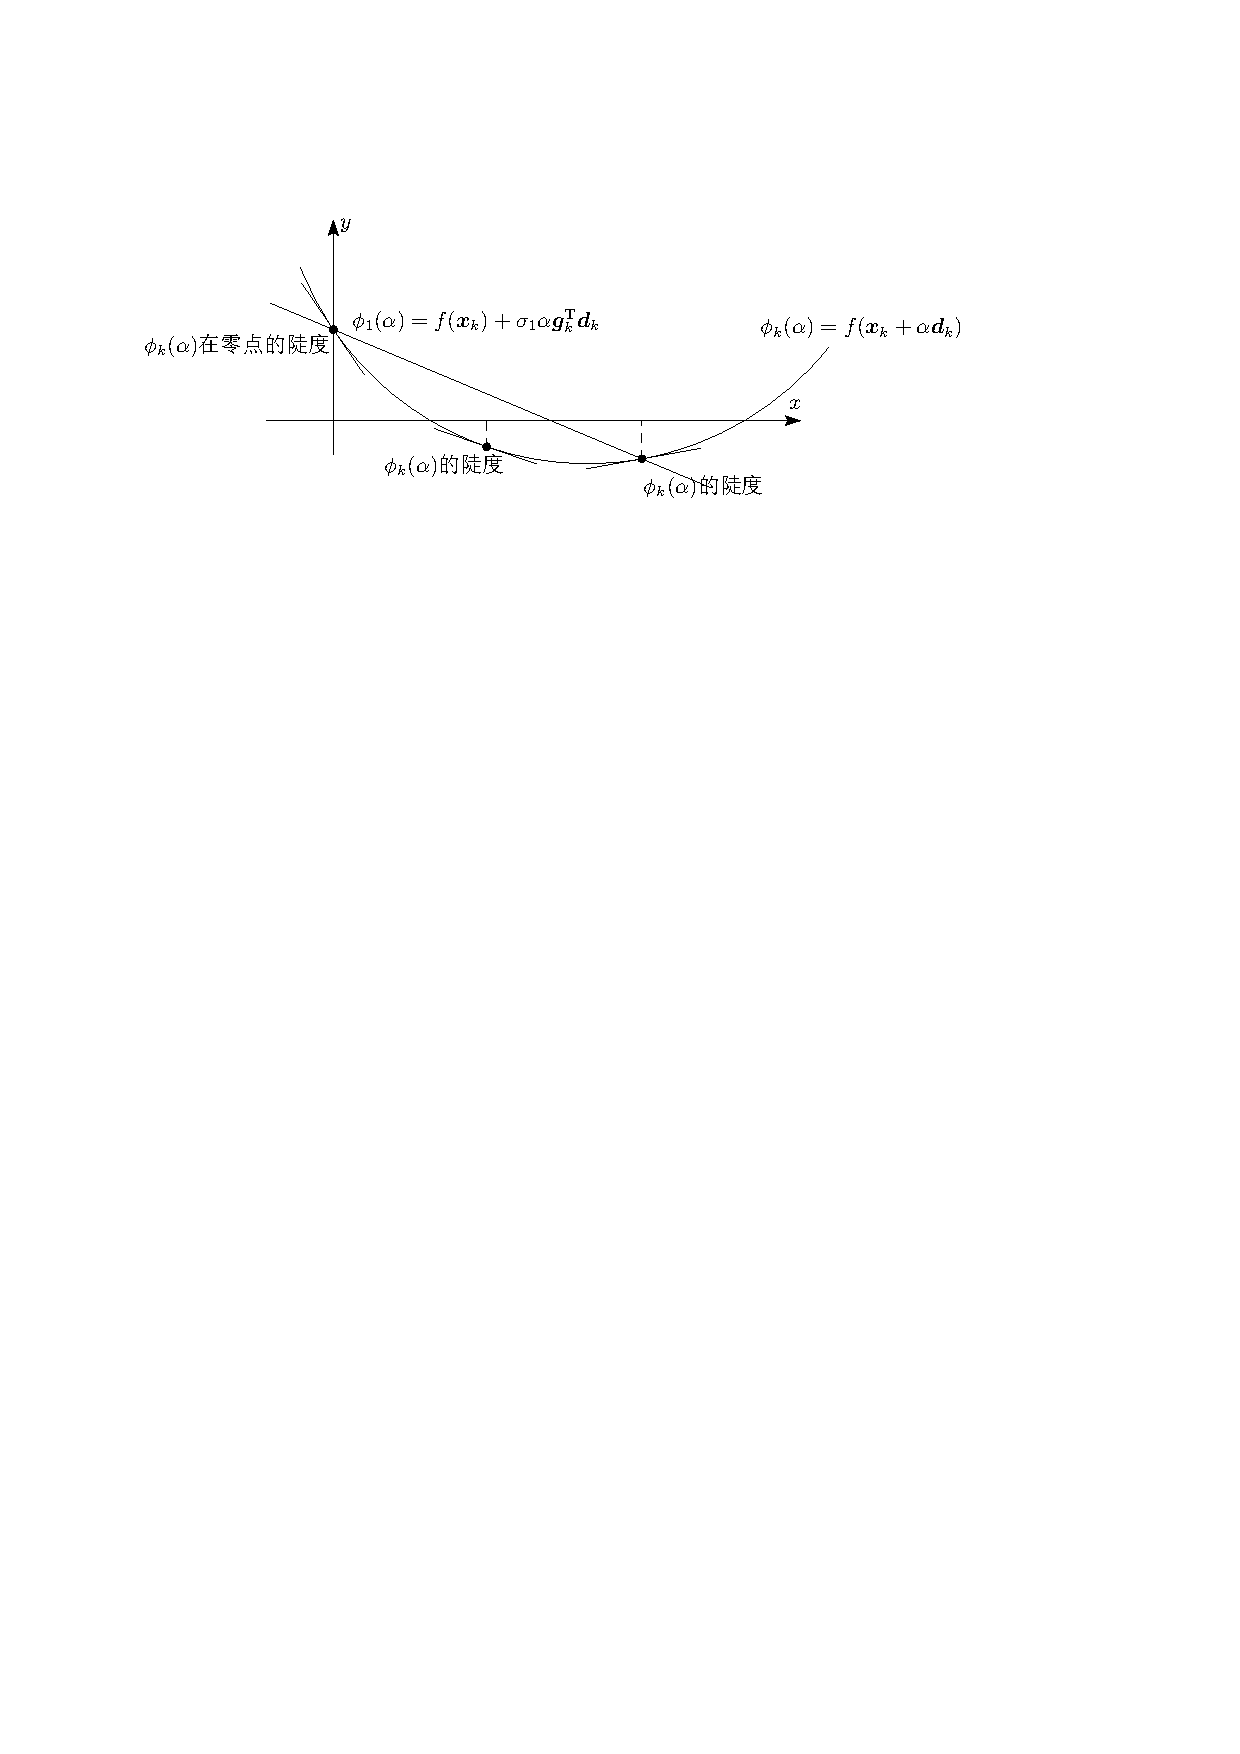
\includegraphics[]{image/Wolfe步长.pdf}
\end{figure}
\subsection{最速算法与牛顿算法}

\subsubsection{最速下降算法}
优化模型$\min\limits_{\boldsymbol{x}\in\mathbb{R}^n}f(\boldsymbol{x})$

迭代算法
\[
    \begin{array}{c}
        \boldsymbol{x}_{k+1} = \boldsymbol{x}_{k} + \alpha_{k}\boldsymbol{d}_{k} \\
        \alpha_{k} = \arg\min\limits_{\alpha\in \mathbb{R}_{+}}f(\boldsymbol{x}_k+\alpha\boldsymbol{d}_k)\\
        \boldsymbol{d}_{k} = -\nabla f(\boldsymbol{x}_k)
    \end{array}  
\]
\begin{corollary}[最优步长规则下的收敛性质]
    最优步长规则下的收敛性质$\boldsymbol{d}_{k}^{\mathrm{T}}\boldsymbol{d}_{k+1} = 0$
\end{corollary}
\begin{proof}
    记$\varphi_k(\alpha)=f(\boldsymbol{x}_k+\alpha\boldsymbol{d}_k).$,利用最优步长规则
    \[
        \begin{aligned}
            0 & =\varphi_{k}^{\prime}(\alpha_{k})=\langle\nabla f(x_{k}+\alpha_{k}\boldsymbol{d}_{k}),\boldsymbol{d}_{k}\rangle   \\
            &=\langle\nabla f(\boldsymbol{x}_{k+1}),\boldsymbol{d}_k\rangle  \\
            &=-\langle\boldsymbol{d}_{k+1},\boldsymbol{d}_{k}\rangle.
        \end{aligned}
    \]
\end{proof}
\begin{theorem}[收敛速度估计]
    对严格凸二次函数$f(\boldsymbol{x}) = \dfrac{1}{2}\boldsymbol{xG}{\mathrm{T}}\boldsymbol{x}$,$\lambda_1\geqslant\lambda_2\geqslant\cdots\geqslant \lambda_n>0$为矩阵$\boldsymbol{G}$的特征根。则最优步长最速下降算法线性收敛,即
    \[
        \frac{f_{k+1}-f(\boldsymbol{x}^*)}{f_k-f(\boldsymbol{x}^*)}\leqslant\Big(\frac{\lambda_1-\lambda_n}{\lambda_1+\lambda_n}\Big)^2,\quad \frac{\lVert\boldsymbol{x}_{k+1}-\boldsymbol{x}^*\rVert}{\lVert\boldsymbol{x}_k-\boldsymbol{x}^*\rVert}\leqslant\frac{\lambda_1-\lambda_n}{\lambda_1+\lambda_n}\sqrt{\frac{\lambda_1}{\lambda_n}}.
    \]
    \begin{itemize}
        \item  很强条件下(二次严格凸)最速下降算法的收敛速度估计;
        \item  线性收敛是一个很慢的收敛速度;
        \item 有例为证:该理论估计是准确的,没有提升的空间。
    \end{itemize}
\end{theorem}
\begin{example}
    $\min\limits_{\boldsymbol{x}\in\mathbb{R}^2}f(x_1,x_2) = \dfrac{1}{3}x_{1}^2+\dfrac{1}{2}x_2^2$。\Stars{5}
    
    显然,唯一最优解$\boldsymbol{x}^* = \left( 0,0 \right)$,取初始点$\boldsymbol{x}_0 = (3,2)$,那么最速下降方法产生的迭代点列
    $\boldsymbol{d}_0$
    \[
        \boldsymbol{x}_{k}=\left(\frac{3}{5^{k}};(-1)^{k}\frac{2}{5^{k}}\right)\overset{k\to\infty}{\longrightarrow}(0;0)
    \]
    全局收敛,收敛速度线性!
    有$\|\boldsymbol{x}_k-\boldsymbol{x}^*\|=\sqrt{13}\big(\frac15\big)^k.$那么
    \[
        \begin{aligned}
            \frac{\|\boldsymbol{x}_{k+1}-\boldsymbol{x}^*\|}{\|\boldsymbol{x}_k-\boldsymbol{x}^*\|} & =\frac15<\frac15\sqrt{\frac32}=\frac{\lambda_1-\lambda_2}{\lambda_1+\lambda_2}\sqrt{\frac{\lambda_1}{\lambda_2}}\\
            \frac{f(\boldsymbol{x}_{k+1})-f(\boldsymbol{x}^*)}{f(\boldsymbol{x}_k)-f(\boldsymbol{x}^*)} & =\frac1{25}=\left(\frac{\lambda_1-\lambda_2}{\lambda_1+\lambda_2}\right)^2
        \end{aligned}
    \]
\end{example}
\begin{note}
    优点:
    \begin{itemize}
        \item 迭代过程简单,计算量与存储量小;
        \item 初始步函数值下降较快,可以快速靠近最优解。
    \end{itemize}

    缺点:
    \begin{itemize}
        \item 相邻两搜索方向正交,导致锯齿现象:越靠近最优值点,靠近速度越慢。
        \item 不适于算法收局。
    \end{itemize}
\end{note}

\subsubsection{牛顿算法}
\[
    \min\limits_{\boldsymbol{x}\in\mathbb{R}^n}f(\boldsymbol{x})
\]
利用目标函数$f(\boldsymbol{x}_k+\boldsymbol{d})$在$\boldsymbol{x}_k$的二阶近似求新的迭代点
\[
    m_k(\boldsymbol{d})\triangleq f(\boldsymbol{x}_k)+\boldsymbol{d}^\mathrm{T}\boldsymbol{g}_k+\frac{1}{2}\boldsymbol{d}^\mathrm{T}\boldsymbol{G}_k\boldsymbol{d}.
\]
利用最优性条件
\[
    \nabla_{\boldsymbol{d}} m_{k}(\boldsymbol{d}) = \boldsymbol{g}_{k}+\boldsymbol{G}_{k}\boldsymbol{d} = \boldsymbol{0} \longrightarrow \boldsymbol{d}_{k}^{N} = -\boldsymbol{G}_{k}^{-1}\boldsymbol{g}_{k}  
\]
令$\boldsymbol{x}_{k+1} = \boldsymbol{x}_{k}-\boldsymbol{G}_{k}^{-1}\boldsymbol{g}_{k}$,即得牛顿算法。牛顿步
\[
    \boldsymbol{d}_{k}^{N} = -\boldsymbol{G}_{k}^{-1}\boldsymbol{g}_{k}
\]
\begin{theorem}
    设目标函数二阶连续可微,Hesse阵在最优值点$\boldsymbol{x}^*$非奇异.则
    \begin{enumerate}
        \item 若初始点充分靠近最优值点,则算法超线性收敛,$\lim\limits_{k\to\infty}\boldsymbol{x}_{k} = \boldsymbol{x}^*$                          
        \item 若Hesse阵在最优值点附近Lipschitz连续, 则二阶收敛。
    \end{enumerate}
\end{theorem}
\begin{proof}
    利用目标函数二阶展式
    \[
        \mathbf{0}=\boldsymbol{g}(x^*)=\boldsymbol{g}_k+\boldsymbol{G}_k(x^*-\boldsymbol{x}_k)+o(\|\boldsymbol{x}_k-\boldsymbol{x}^*\|).
    \]
    左乘$\boldsymbol{G}_{k}^{-1}$
    \[
        \begin{array}{l}
            \boldsymbol{x}_k-\boldsymbol{x}^*-\boldsymbol{G}_k^{-1}\boldsymbol{g}_k=o(\|\boldsymbol{x}_k-\boldsymbol{x}^*\|)\\
            \Rightarrow \boldsymbol{x}_{k+1}-\boldsymbol{x}^{*}=o(\|\boldsymbol{x}_{k}-\boldsymbol{x}^{*}\|). 
        \end{array}
    \]
    证毕!
\end{proof}
\begin{note}
    算法特点:
    \begin{itemize}
        \item 无全局收敛性。仅局部收敛,即要求初始点靠近最优值点;
        \item 二阶收敛:迭代点越靠近最优值点, 收敛速度越快!
        \item 具有二次终止性:对严格凸二次函数,一步即得最优解
        \item 严格二次函数$f(\boldsymbol{x})=\frac12\boldsymbol{x}^{\mathrm{T}}\boldsymbol{G}\boldsymbol{x}+\boldsymbol{g}^{\mathrm{T}}\boldsymbol{x}+c\Rightarrow \boldsymbol{x}^* = -\boldsymbol{G}^{-1}\boldsymbol{g}$
        
        任意初始点$\boldsymbol{x}_{0}\in\mathbb{R}^n$
        \[
            \begin{aligned}
                \boldsymbol{x}_{1}& =\boldsymbol{x}_{0}-G^{-1}\nabla f(\boldsymbol{x}_{0})  \\
                &=\boldsymbol{x}_{0}-\boldsymbol{G}^{-1}(\boldsymbol{G}\boldsymbol{x}_{0}+\boldsymbol{g}) \\
                &=-\boldsymbol{G}^{-1}\boldsymbol{g}=\boldsymbol{x}^{*}.
            \end{aligned}
        \]
    \end{itemize}
\end{note}
\begin{example}
    用牛顿法求解$\min f(x)=\sqrt{1+x^2}$\quad\Stars{5}
    
    $0$为最优解
    
    目标函数导数$f'(x)=\dfrac{x}{\sqrt{1+x^2}}\quad f''(x)=\dfrac{1}{(1+x^2)^{3/2}}$
    
    迭代过程
    \[
        \begin{aligned}
            x_{k+1}& =x_{k}-\frac{f'(x_{k})}{f''(x_{k})}  \\
            &=x_{k}-x_{k}(1+x_{k}^{2}) \\
            &=-x_{k}^{3}
        \end{aligned}
    \]
    \begin{itemize}
        \item 当$x_0<1$,算法快速收敛到最优解;
        \item 当$x_0\geqslant 1$,算法不收敛
    \end{itemize}
\end{example}
% \begin{example}
%     用牛顿算法求解$\operatorname*{min}f(\boldsymbol{x})=4x_{1}^{2}+x_{2}^{2}-x_{1}^{2}x_{2}$

%     目标函数梯度信息
%     \[
%         \nabla f(\boldsymbol{x})=\begin{pmatrix}8x_1-2x_1x_2\\2x_2-x_1^2\end{pmatrix}\quad\nabla^2f(\boldsymbol{x})=\begin{pmatrix}8-2x_2&-2x_1\\-2x_1&2\end{pmatrix}
%     \]
% \end{example}
\begin{note}
    牛顿方法的缺陷
    \begin{itemize}
        \item 初始点远离最优解时,算法可能不收敛;
        \item Hesse矩阵奇异时,算法不可行;
        \item  计算量和存储量大:需计算目标函数的梯度和Hesse阵
    \end{itemize}
\end{note}

\subsection{共轭梯度法}
线性方程组($\boldsymbol{A}$对称正定):
\[
    \boldsymbol{Ax} = \boldsymbol{b}
\]
\begin{itemize}
    \item 经典算法:Gauss消元法、系数矩阵三角分解法
    \item 算法缺陷:计算时间随问题规模急速增长。
\end{itemize}

将问题转化为
\[
    \min f(\boldsymbol{x}) = \dfrac{1}{2}\boldsymbol{x}^{\mathrm{T}}\boldsymbol{Ax}-\boldsymbol{b}^{\mathrm{T}}\boldsymbol{x}
\]

\subsubsection{线性共轭方向法}

\begin{definition}[共轭方向]
    对对称正定阵$\boldsymbol{A}$,若$\boldsymbol{d}_1,\boldsymbol{d}_2\in\mathbb{R}^n$,满足$\boldsymbol{d}_{1}^{\mathrm{T}}\boldsymbol{Ad}_2 = 0$,则称$\boldsymbol{d}_1,\boldsymbol{d}_2$关于矩阵$\boldsymbol{A}$共轭,并称其为$A$的共轭方向。

    \textcolor{red}{共轭是正交的推广。}
\end{definition}

\begin{definition}[线性共轭方向的推广]
    若向量组$\boldsymbol{d}_1,\boldsymbol{d}_2,\cdots,\boldsymbol{d}_n$关于对称正定阵$\boldsymbol{A}$两两共轭,即满足
    \[
        \boldsymbol{d}_i\boldsymbol{A}\boldsymbol{d}_j  = 0,\,1\leqslant i\neq j\leqslant k
    \]
\end{definition}
\begin{corollary}
    若向量组$\boldsymbol{d}_1,\boldsymbol{d}_2,\cdots,\boldsymbol{d}_n$,关于矩阵$\boldsymbol{A}$共轭,则它们线性无关。
\end{corollary}

\begin{note}
    线性共轭方向法:
    \[
    \min\limits_{\boldsymbol{x}\in\mathrm{R}^n} f(\boldsymbol{x}) = \dfrac{1}{2}\boldsymbol{x}^{\mathrm{T}}\boldsymbol{Ax}-\boldsymbol{b}^{\mathrm{T}}x
    \]
    \begin{enumerate}
        \item 初始点$\boldsymbol{x}_0$,搜索方向$\boldsymbol{d}_0$满足$\left< \boldsymbol{d}_0,\boldsymbol{g}_0 \right><0$,终止参数$\varepsilon\geqslant 0$,令$k=0$
        \item 若$\|\boldsymbol{g}_k\|\leqslant \varepsilon$,算法终止;否则,进入下一步
        \item 计算最优步长$\alpha = \arg\min\limits_{\alpha\geqslant 0}\left\{ f(\boldsymbol{x}_k+\alpha \boldsymbol{d}_{k}) \right\}$,令$\boldsymbol{x}_{k+1} = \boldsymbol{x}_k+\alpha_k\boldsymbol{d}_k$
        \item 构造$\boldsymbol{d}_{k+1}$使其与$\boldsymbol{d}_0,\cdots,\boldsymbol{d}_k$关于矩阵$\boldsymbol{A}$共轭,令$k \gets k+1$,返回步2
    \end{enumerate}
\end{note}

\begin{theorem}[二次终止性]
    对严格凸二次函数$\min f(\boldsymbol{x}) = \dfrac{1}{2}\boldsymbol{x}^{\mathrm{T}}\boldsymbol{Ax}-\boldsymbol{b}^{\mathrm{T}}\boldsymbol{x}$,向量组$\boldsymbol{d}_0,\boldsymbol{d}_1,\cdots,\boldsymbol{d}_{n-1}$关于$\boldsymbol{A}$共轭。共轭方向发产生点列$\left\{ \boldsymbol{x}_{k} \right\}$。则对任意$0\leqslant k\leqslant n-1$,$\boldsymbol{x}_{k+1}$是目标函数在仿射集$\boldsymbol{x}_0+\operatorname{span}\left[ \boldsymbol{d}_0,\cdots,\boldsymbol{d}_{k} \right]$上的最小值点,算法至多$n$步迭代后终止。
\end{theorem}
\begin{example}
    利用共轭梯度法求$\boldsymbol{Ax} = \boldsymbol{b}$或者说,利用共轭梯度法求$\min x_1^2+\dfrac{1}{2}x_2^2+\dfrac{1}{2}x_3^2$\quad\Stars{5}


    其中,
    \[
        \boldsymbol{A} = \begin{bmatrix}
            1 & 0 & 0\\
            0 & \frac{1}{2} & 0 \\
            0 & 0 & \frac{1}{2}
        \end{bmatrix},\quad
        \boldsymbol{b} = \begin{pmatrix}
            0\\0\\0
        \end{pmatrix}
    \]

    解:

    
    取初始点$\boldsymbol{x}_0 = (1,1,1)^{\mathrm{T}} $,迭代过程:
    \begin{enumerate}
        \item $\boldsymbol{x}_0 = (1,1,1)^{\mathrm{T}} $,$\boldsymbol{g}_0 = \boldsymbol{Ax}_0-\boldsymbol{0} = (2,1,1)^{\mathrm{T}}$,$\beta_{-1} = 0$,$\boldsymbol{d}_{0} = -\boldsymbol{g}_0$.
        \[
            \begin{array}{ll}
                \alpha &= \arg\min f(\boldsymbol{x}_0+\alpha \boldsymbol{d}_0)\\
                & = (1-2\alpha)^2+\frac{1}{2}(1-\alpha)^2+\frac{1}{2}(1-\alpha)^2 = \frac{3}{5}
            \end{array}
        \]
        \item $\boldsymbol{x}_1 = \boldsymbol{x}_0+\alpha_0\boldsymbol{d}_0=\frac{1}{5}(-1,2,2)^{\mathrm{T}} $,$\boldsymbol{g}_0 = \boldsymbol{Ax}_1-\boldsymbol{0} = \frac{1}{5}(-1,2,2)^{\mathrm{T}}$,$\beta_{0} = \frac{\boldsymbol{g}_1^{\mathrm{T}}\boldsymbol{g}_1}{\boldsymbol{g}_0^{\mathrm{T}}\boldsymbol{g}_0}= \frac{2}{25}$ 
        \[
            \boldsymbol{d}_{1} = -\boldsymbol{g}_1+\beta_{0}\boldsymbol{g}_0 = -\frac{6}{25}(1,-2,-2)^{\mathrm{T}}
        \]
        \[
            \begin{array}{ll}
                \alpha &= \arg\min f(\boldsymbol{x}_0+\alpha \boldsymbol{d}_0)\\
                & = (1-2\alpha)^2+\frac{1}{2}(1-\alpha)^2+\frac{1}{2}(1-\alpha)^2 = \frac{3}{5}
            \end{array}
        \]
        \item $\boldsymbol{x}_2 = \boldsymbol{x}_1 + \alpha_1\boldsymbol{d}_1 = \boldsymbol{0}$,$\|\boldsymbol{g}_2\| = 0$,终止。
    \end{enumerate}

    \begin{table}[htbp]
        \centering
        \begin{tabular}{c|c|c|c|c|c}
            \hline
            $k$ & $\boldsymbol{x}_k$ & $\boldsymbol{g}_k$ & $\beta_{k-1}$ & $\boldsymbol{d}_k$ & $\alpha_k$\\\hline
            $0$ & $ (1,1,1)^{\mathrm{T}} $ & $(2,1,1)^{\mathrm{T}}$ & $0$ & $ -(2,1,1)^{\mathrm{T}} $ & $\frac{3}{5}$\\\hline
            $1$ & $ \frac{1}{5}(-1,2,2)^{\mathrm{T}} $ & $\frac{1}{5}(-2,2,2)^{\mathrm{T}}$ & $\frac{2}{25}$ & $ -\frac{6}{25}(1,-2,-2)^{\mathrm{T}} $ & $\frac{5}{6}$\\\hline
            $2$ & $(0,0,0)^{\mathrm{T}}$ & $(0,0,0)^{\mathrm{T}}$ & \\\hline
        \end{tabular}
    \end{table}
\end{example}
\begin{theorem}[收敛速度]
    对严格凸二次函数$f(\boldsymbol{x}) = \dfrac{1}{2}\boldsymbol{x}^{\mathrm{T}}\boldsymbol{Ax}-\boldsymbol{b}^{\mathrm{T}}\boldsymbol{x}$.若系数矩阵$\boldsymbol{A}$有$r$个相异特征根,则最优步长规则下的共轭梯度法至多$r$步迭代后终止。
\end{theorem}

\subsection{拟牛顿算法}
\begin{note}
    基本思想:利用已产生迭代点的梯度信息构造目标函数Hesse矩阵的一个近似,进而建立牛顿方向的一个近似,再通过线搜索产生新的迭代点。
    \begin{figure}[htbp]
        \centering
        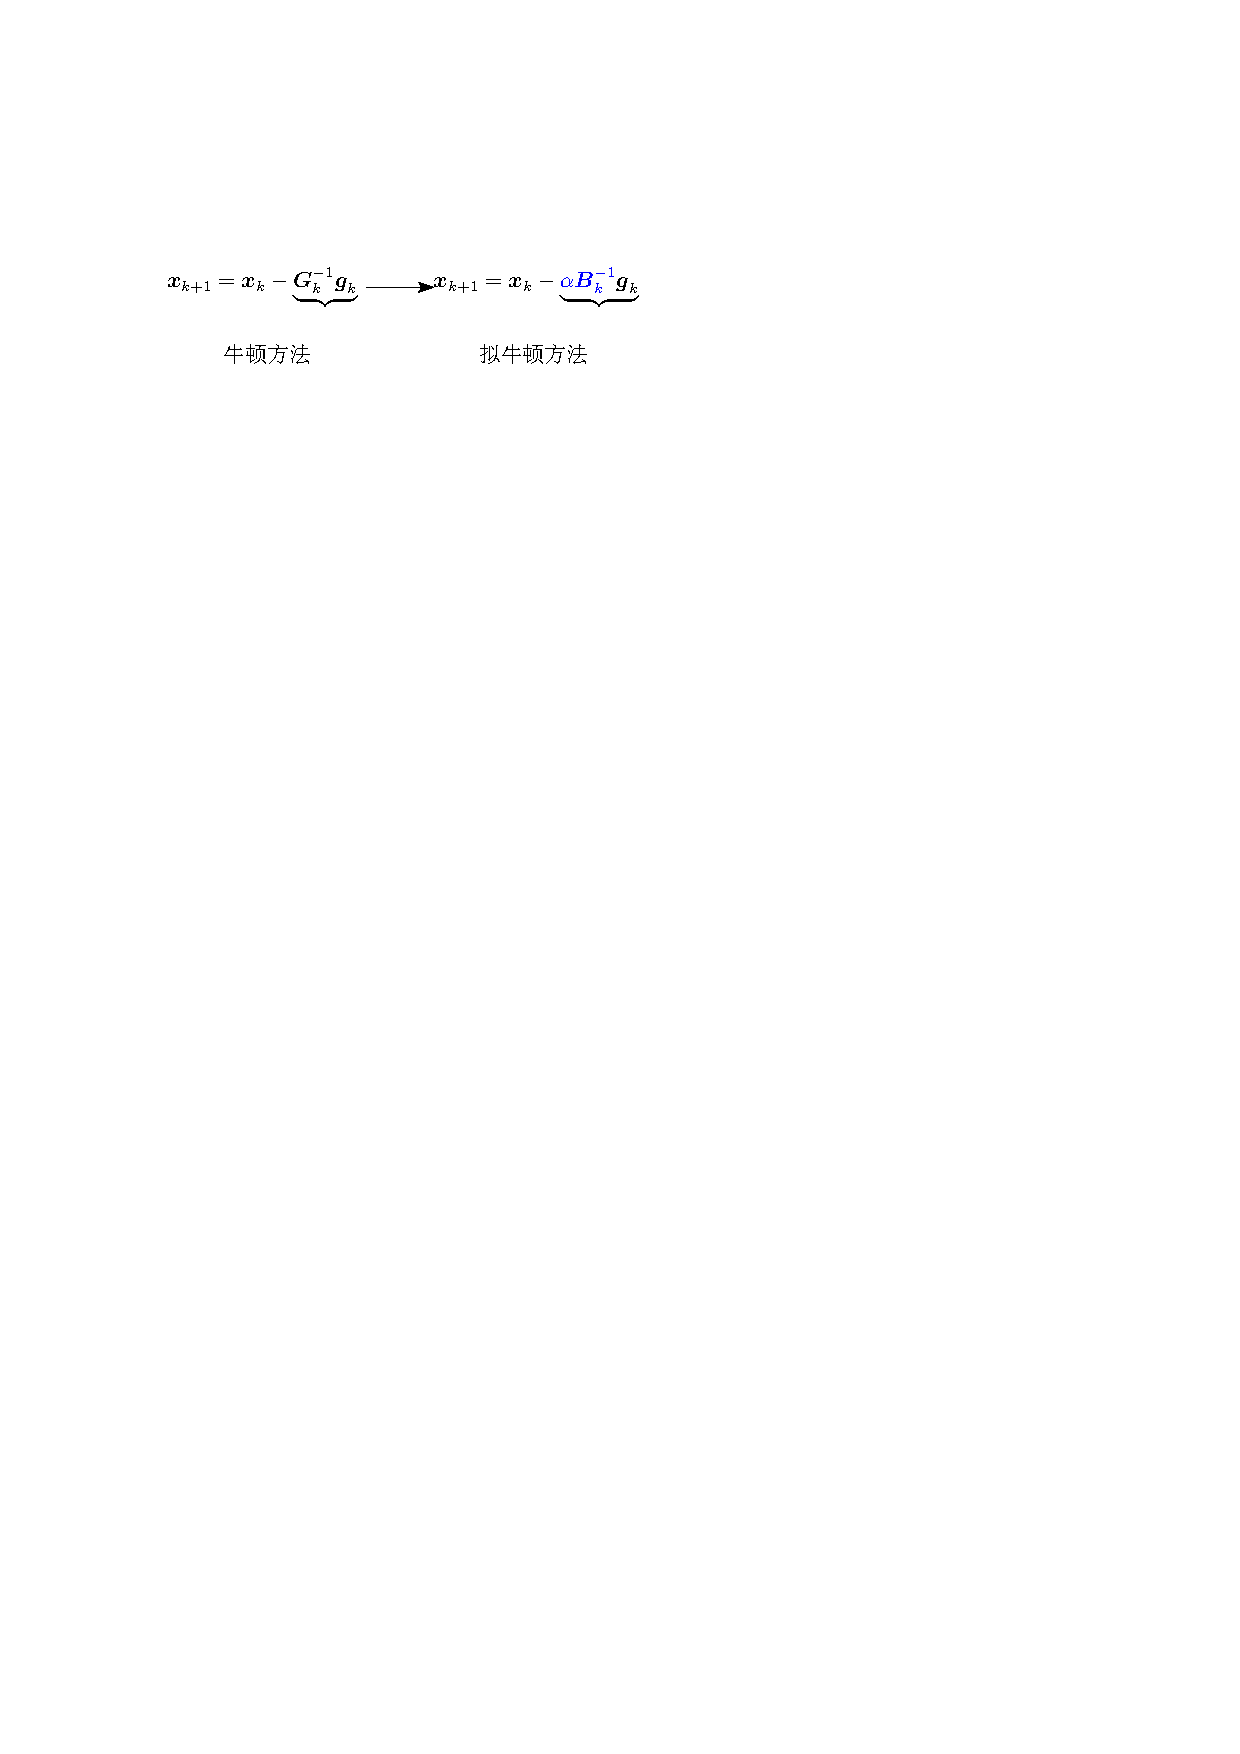
\includegraphics{image/拟牛顿方程.pdf}
    \end{figure}
\end{note}
考察目标函数梯度$\boldsymbol{g}(\boldsymbol{x})$在$\boldsymbol{x}_{k+1}$点的线性近似
\[
    \begin{array}{cl}
        & \boldsymbol{g}(\boldsymbol{x}_k)\approx \boldsymbol{g}_{k+1}+\boldsymbol{G}_{k+1}(\boldsymbol{x}_k-\boldsymbol{x}_{k+1})\\
        \implies   & \boldsymbol{g}_{k+1} - \boldsymbol{g}_{\boldsymbol{x}_k}\approx \boldsymbol{G}_{k+1}(\boldsymbol{x}_{k+1}-\boldsymbol{x}_k)\\
        \overset{\colorbox{blue!25}{$\begin{array}{l}
            \boldsymbol{y}_{k} = \boldsymbol{g}_{k+1}-\boldsymbol{g}_{k}\\
            \boldsymbol{s}_{k} = \boldsymbol{x}_{k+1}-\boldsymbol{x}_{k}
        \end{array}$}}{\implies} & \boldsymbol{y}_{k}\approx \boldsymbol{G}_{k+1}\boldsymbol{s}_{k}\\
        \overset{\boldsymbol{H}_{k+1} = \boldsymbol{B}_{k+1}^{-1}}{\implies} & \boldsymbol{H}_{k+1}\boldsymbol{y}_{k}\approx \boldsymbol{s}_{k}
    \end{array}
\]

得到重要结论
\[
    \textcolor{red}{\boldsymbol{H}_{k+1}\boldsymbol{y}_{k}\approx \boldsymbol{s}_{k}}
\]
\subsubsection{对称秩-1校正公式}
\begin{note}
    对称秩-1校正公式:
    \[
        \boldsymbol{H}_{k+1} = \boldsymbol{H}_{k} + \boldsymbol{v}_k\boldsymbol{v}_{k}^{\mathrm{T}}
    \]
    使用$\boldsymbol{H}_{k+1}\boldsymbol{y}_{k}\approx \boldsymbol{s}_{k}$两边同时乘以$\boldsymbol{y}_{k}$得到
    \[
        \boldsymbol{H}_{k}\boldsymbol{y}_{k} + \boldsymbol{v}_k\boldsymbol{v}_{k}^{\mathrm{T}}\boldsymbol{y}_{k} = \boldsymbol{s}_{k}
    \]
    得到
    \[
        \boldsymbol{v}_k = \dfrac{\boldsymbol{s}_{k}-\boldsymbol{H}_{k}\boldsymbol{y}_{k}}{\boldsymbol{v}_{k}^{\mathrm{T}}\boldsymbol{y}_{k}}
    \]
    所以对于$\boldsymbol{v}_k\boldsymbol{v}_{k}^{\mathrm{T}}$有
    \[
        \begin{array}{ll}
            \boldsymbol{v}_k\boldsymbol{v}_{k}^{\mathrm{T}} &= \dfrac{(\boldsymbol{s}_{k}-\boldsymbol{H}_{k}\boldsymbol{y}_{k})(\boldsymbol{s}_{k}-\boldsymbol{H}_{k}\boldsymbol{y}_{k})^\mathrm{T}}{(\boldsymbol{v}_{k}^{\mathrm{T}}\boldsymbol{y}_{k})(\boldsymbol{y}_{k}^{\mathrm{T}}\boldsymbol{v}_{k})}\\
            &=\dfrac{(\boldsymbol{s}_{k}-\boldsymbol{H}_{k}\boldsymbol{y}_{k})(\boldsymbol{s}_{k}-\boldsymbol{H}_{k}\boldsymbol{y}_{k})^\mathrm{T}}{\boldsymbol{y}_{k}^{\mathrm{T}}\boldsymbol{v}_{k}\boldsymbol{v}_{k}^{\mathrm{T}}\boldsymbol{y}_{k}}\\
            &=\dfrac{(\boldsymbol{s}_{k}-\boldsymbol{H}_{k}\boldsymbol{y}_{k})(\boldsymbol{s}_{k}-\boldsymbol{H}_{k}\boldsymbol{y}_{k})^\mathrm{T}}{(\boldsymbol{s}_{k}-\boldsymbol{H}_{k}\boldsymbol{y}_{k})^\mathrm{T}\boldsymbol{y}_{k}}
        \end{array}
    \]
    故而,
    \begin{equation}\label{eq:Rank-1_Hk+1}
        \boldsymbol{H}_{k+1} = \boldsymbol{H}_{k} + \dfrac{(\boldsymbol{s}_{k}-\boldsymbol{H}_{k}\boldsymbol{y}_{k})(\boldsymbol{s}_{k}-\boldsymbol{H}_{k}\boldsymbol{y}_{k})^\mathrm{T}}{(\boldsymbol{s}_{k}-\boldsymbol{H}_{k}\boldsymbol{y}_{k})^\mathrm{T}\boldsymbol{y}_{k}}
    \end{equation}
    \begin{enumerate}
        \item 取$\boldsymbol{x}_{0}\in\mathbb{R}^{n}$,矩阵$\boldsymbol{H}_{0}$(一般取$\boldsymbol{H}_{0} = \boldsymbol{I}$)和计算精度$\varepsilon$,令$k = 0$
        \item 计算搜索方向$\boldsymbol{d}_{k} = -\boldsymbol{H}_{k}\boldsymbol{g}_k$。令$\boldsymbol{x}_{k+1} = \boldsymbol{x}_{k}+\alpha_k\boldsymbol{d}_k$。其中, 步长由线搜索产生. 若$\|\boldsymbol{g}_{k+1}\|\leqslant \varepsilon$,算法停止;否则转下一步
        \item 利用
        \[
            \boldsymbol{H}_{k+1} = \boldsymbol{H}_{k} + \dfrac{(\boldsymbol{s}_{k}-\boldsymbol{H}_{k}\boldsymbol{y}_{k})(\boldsymbol{s}_{k}-\boldsymbol{H}_{k}\boldsymbol{y}_{k})^\mathrm{T}}{(\boldsymbol{s}_{k}-\boldsymbol{H}_{k}\boldsymbol{y}_{k})^\mathrm{T}\boldsymbol{y}_{k}}
        \]
        计算$\boldsymbol{H}_{k+1}$,令$k = k+1$,转步2
    \end{enumerate}
\end{note}
\subsubsection{DFP校正公式}
\begin{note}
    DFP校正公式:

    基于对称秩-1校正公式中的校正项
    \[
        \boldsymbol{H}_{k+1} = \boldsymbol{H}_{k} + \dfrac{(\textcolor{cyan!75}{\boldsymbol{s}_{k}}-\textcolor{blue!75}{\boldsymbol{H}_{k}\boldsymbol{y}_{k}})(\boldsymbol{s}_{k}-\boldsymbol{H}_{k}\boldsymbol{y}_{k})^\mathrm{T}}{(\boldsymbol{s}_{k}-\boldsymbol{H}_{k}\boldsymbol{y}_{k})^\mathrm{T}\boldsymbol{y}_{k}}
    \]
    对$\boldsymbol{H}_{k}$做如下对称秩-2校正
    \[
        \boldsymbol{H}_{k+1} = \boldsymbol{H}_{k} + a\textcolor{cyan!75}{\boldsymbol{s}_{k}\boldsymbol{s}_{k}^{\mathrm{T}}}+b\textcolor{blue!75}{\boldsymbol{H}_{k}\boldsymbol{y}_{k}\boldsymbol{y}_{k}^{\mathrm{T}}\boldsymbol{H}_{k}}
    \]
    利用$\textcolor{red}{\boldsymbol{H}_{k+1}\boldsymbol{y}_{k} = \boldsymbol{s}_{k}}$
    得到
    \[
        \cancel{\boldsymbol{H}_{k}\boldsymbol{y}_{k}} + a\textcolor{cyan!75}{\underline{\boldsymbol{s}_{k}}\boldsymbol{s}_{k}^{\mathrm{T}}}\boldsymbol{y}_{k}+\cancel{b\textcolor{blue!75}{\boldsymbol{H}_{k}\boldsymbol{y}_{k}\boldsymbol{y}_{k}^{\mathrm{T}}\boldsymbol{H}_{k}}\boldsymbol{y}_{k} } = \underline{\boldsymbol{s}_{k}}
    \]
    两边相等,故而
    \[
        a = \dfrac{1}{\boldsymbol{s}_{k}^{\mathrm{T}}\boldsymbol{y}_{k}},\quad b = -\dfrac{1}{\boldsymbol{y}_{k}^{\mathrm{T}}\boldsymbol{H}_{k}\boldsymbol{y}_{k}} 
    \]
    故而得到DFP校正公式
    \[
        \boldsymbol{H}_{k+1} = \boldsymbol{H}_{k} + \dfrac{\textcolor{cyan!75}{\boldsymbol{s}_{k}\boldsymbol{s}_{k}^{\mathrm{T}}}}{\boldsymbol{s}_{k}^{\mathrm{T}}\boldsymbol{y}_{k}} - \dfrac{\textcolor{blue!75}{\boldsymbol{H}_{k}\boldsymbol{y}_{k}\boldsymbol{y}_{k}^{\mathrm{T}}\boldsymbol{H}_{k}}}{\boldsymbol{y}_{k}^{\mathrm{T}}\boldsymbol{H}_{k}\boldsymbol{y}_{k}}
    \]
\end{note}


\begin{example}
    用DFP方法求解优化问题\Stars{5}{}
    \[
        \min f(\boldsymbol{x})=2x_{1}^{2}+x_{2}^{2}-4x_{1}+2
    \]
    解:容易计算$\boldsymbol{x}^* = (1,0)^{\mathrm{T}}$
    \[
        \nabla f(\boldsymbol{x}) = \begin{pmatrix}
            4x_1-4\\
            2x_2
        \end{pmatrix}
    \]
    \begin{enumerate}
        \item 取初始值$\boldsymbol{x}_0 = (2,1)^{\mathrm{T}}$,$\boldsymbol{H}_0 = \boldsymbol{I}$,则$\boldsymbol{g}_0 = (4,2)^{\mathrm{T}}$,沿着$\boldsymbol{d}_0 = -\boldsymbol{H}_0\boldsymbol{g}_0 = (-4,-2)^{\mathrm{T}}$精确线搜索得到$\alpha = \dfrac{5}{18}$
        
        新迭代点$\boldsymbol{x}_1 = \boldsymbol{x}_0+\alpha\boldsymbol{d}_0 = (\dfrac{8}{9},\dfrac{4}{9})^{\mathrm{T}}$
        进入下一次迭代
        \item 计算$\boldsymbol{x}_1 = \boldsymbol{x}_0+\alpha\boldsymbol{d}_0 = (\dfrac{8}{9},\dfrac{4}{9})^{\mathrm{T}}$,梯度$\boldsymbol{g}_0 = (-\dfrac{4}{9},\dfrac{8}{9})^{\mathrm{T}}$,进而计算
        \[
            \begin{aligned}
                \boldsymbol{s}_0&= \boldsymbol{x}_{1}-\boldsymbol{x}_{0} =\alpha_0\boldsymbol{d}_0=(-\frac{10}{9},-\frac{5}{9})^{\mathrm{T}}\\ 
                \boldsymbol{y}_0&=\boldsymbol{g}_1-\boldsymbol{g}_0=(-\frac{40}{9},-\frac{40}{9})^{\mathrm{T}}
            \end{aligned}
        \]
        得校正矩阵
        \[
            \boldsymbol{H}_1=\boldsymbol{H}_{0} + \dfrac{\textcolor{cyan!75}{\boldsymbol{s}_{0}\boldsymbol{s}_{0}^{\mathrm{T}}}}{\boldsymbol{s}_{0}^{\mathrm{T}}\boldsymbol{y}_{0}} - \dfrac{\textcolor{blue!75}{\boldsymbol{H}_{0}\boldsymbol{y}_{0}\boldsymbol{y}_{0}^{\mathrm{T}}\boldsymbol{H}_{0}}}{\boldsymbol{y}_{0}^{\mathrm{T}}\boldsymbol{H}_{0}\boldsymbol{y}_{0}}
            =\frac{1}{360}\begin{pmatrix}86&-38\\-38&305\end{pmatrix}
        \]
        沿着$\boldsymbol{d}_1=-\boldsymbol{H}_1\boldsymbol{g}_1=\dfrac{12}{51}(1,-4)^{\mathrm{T}}$精确线搜索得到$\alpha_1 = \dfrac{17}{36}$
        
        新迭代点$\boldsymbol{x}_{2}=\boldsymbol{x}_{1}+\alpha_{1}\boldsymbol{d}_{1}=\left(1,0\right)^{\mathrm{T}}=\boldsymbol{x}^{*}$,算法终止。
    \end{enumerate}
\end{example}

\subsection{信赖域方法}
优化模型$\min\limits_{\boldsymbol{x}\in\mathbb{R}^n}f(x)$

信赖域方法:$\boldsymbol{x}_{k+1}\gets \boldsymbol{x}_{k}$使得$f(\boldsymbol{x}_{k+1})<f(\boldsymbol{x})$

算法思想:构造目标函数的二阶近似,将其在当前点邻域内的最小值点作为新的迭代点。

构造$f(\boldsymbol{x}_k+\boldsymbol{d})$的二阶近似
\[
    m_{k}(\boldsymbol{d})=f(\boldsymbol{x}_{k})+\boldsymbol{g}_{k}^{\mathrm{T}}\boldsymbol{d}+\frac{1}{2}\boldsymbol{d}^{\mathrm{T}}\boldsymbol{B}_{k}\boldsymbol{d}
\]
其中$\boldsymbol{B}_{k}=\nabla^{2}f(\boldsymbol{x}_{k})$或者$\boldsymbol{B}_{k}\approx\nabla^{2}f(\boldsymbol{x}_{k}).$

\begin{note}
    信赖域子问题
    \[
        \min\{m_k(\boldsymbol{d})\mid\boldsymbol{d}\in\mathbb{R}^n,\lVert\boldsymbol{d}\rVert\leqslant\Delta_k\}.
    \]
    其中,$\Delta_{k}>0$为信赖域半径。

    设$\boldsymbol{d}_k$为其最优解。则目标函数与二次模型的近似度为
    \[
        f(\boldsymbol{x}_k+\boldsymbol{d}_k)-m_k(\boldsymbol{d}_k)=O(\|\boldsymbol{d}_k\|^2)
    \]
    若$\boldsymbol{B}_{k}=\nabla^{2}f(\boldsymbol{x}_{k})$,则
    \[
        f(\boldsymbol{x}_k+\boldsymbol{d}_k)-m_k(\boldsymbol{d}_k)=O(\|\boldsymbol{d}_k\|^2)
    \]
\end{note}
\begin{note}
    调整依据:$m_{k}(\boldsymbol{d}_k)$与$f(\boldsymbol{\boldsymbol{x}}_k+\boldsymbol{d}_k)$的近似度

    \begin{itemize}
        \item 预下降量:$\mathrm{Pred}_{k}=m_{k}(\boldsymbol{0})+m_{k}(\boldsymbol{d}_{k}),$
        \item 实下降量:$\mathrm{Ared}_k=f(\boldsymbol{x}_k)-f(\boldsymbol{x}_k+\boldsymbol{d}_k)$
        \item 下降比:$r_{k}={\dfrac{\mathrm{Ared}_{k}}{\mathrm{Pred}_{k}}}$
    \end{itemize}
\end{note}

\begin{note}
    信赖域算法:
    \begin{enumerate}
        \item 取$\hat{\Delta}>0,\boldsymbol{x}_{0}\in\mathbb{R}^{n},\Delta_{0}^{i}\in(0,\hat{\Delta}],\eta\in[0,\frac{1}{4}),\varepsilon\geqslant 0.$令$k = 0$
        \item 若$\|g_k\|\leqslant\varepsilon $,算法终止;否则进入下一步
        \item 解子问题$ \boldsymbol{d}_k=\arg\min\{m_k(\boldsymbol{d})\mid\boldsymbol{d}\in\mathbb{R}^n,\lVert\boldsymbol{d}\rVert\leqslant\Delta_k\} $
        
        计算$r_{k}={\dfrac{\mathrm{Ared}_{k}}{\mathrm{Pred}_{k}}}$

        若$r_{k}<\dfrac{1}{4}.$令$\Delta_{k+1}=\frac{1}{4}\Delta_{k}$;
        
        若$r_{k}>\dfrac34$,且$\|\boldsymbol{d}_{k}\|=\Delta_{k},$令$\Delta_{k+1}=\min\{2\Delta_{k},\hat{\Delta}\}$;

        否则,令$\Delta_{k+1} = \Delta_k$
        \item 若$r_{k}>\eta$,令$\boldsymbol{x}_{k+1} = \boldsymbol{x}_k+\boldsymbol{d}_k$
        
        否则,令$\boldsymbol{x}_{k+1}=\boldsymbol{x}_{k},k=k+1$,转2
    \end{enumerate}
\end{note}

\subsection{最小二乘问题}
最小二乘问题数学模型
\[
    \min\limits_{\boldsymbol{x}\in \mathbb{R}^n}\sum\limits_{i = 1}^{n}\left( y_i-\phi(\boldsymbol{x},t_i) \right)^2
\]
\begin{note}
    模型特点:
    \begin{itemize}
        \item $m\gg n$
        \item 目标函数为平方和形式,函数值非负
        \item 目标函数选取值恰当时,目标函数的最优值靠近零
    \end{itemize}
\end{note}
设$r_i(\boldsymbol{x}) = y_i-\phi(\boldsymbol{x},t_i)$模型可以写为
\[
    \min\limits_{\boldsymbol{x}\in \mathbb{R}^n}\boldsymbol{r}(\boldsymbol{x})^{\mathrm{T}}\boldsymbol{r}(\boldsymbol{x})
\]
其中$\boldsymbol{r}(\boldsymbol{x})=(r_1(\boldsymbol{x}),r_2(\boldsymbol{x}),\cdots,r_m(\boldsymbol{x}))^{\mathrm{T}}$。
\subsubsection{线性最小二乘}
数学模型
\[
    \min_{\boldsymbol{x}\in\mathbb{R}^n}\frac12\boldsymbol{r}(\boldsymbol{x})^{\mathrm{T}}\boldsymbol{r}(\boldsymbol{x})
\]
其中$\boldsymbol{r}(\boldsymbol{x})=\boldsymbol{Ax}-\boldsymbol{b},\boldsymbol{A}\in\mathbb{R}^{m\times n},\boldsymbol{b}\in\mathbb{R}^m$
问题转换为
\[
    \min_{\boldsymbol{x}\in\mathbb{R}^n}\frac12\|\boldsymbol{Ax}-\boldsymbol{b}\|^2
\]
\begin{theorem}
    线性最小二乘问题存在全局最优解。它有唯一最优解的充分必要条件是矩阵$\boldsymbol{A}$列满秩。
\end{theorem}
\subsubsection{非线性最小二乘}
数学模型
\[
    \min\limits_{\boldsymbol{x}\in \mathbb{R}^n} f(\boldsymbol{x}):=\frac12{\left\|\boldsymbol{r}(\boldsymbol{x})\right\|}^{2}
\]
\begin{note}
    梯度
    \[
        \nabla f(\boldsymbol{x})=\boldsymbol{g}(\boldsymbol{x})=\nabla\Bigl(\frac{1}{2}\boldsymbol{r}(\boldsymbol{x})^{\mathrm{T}}\boldsymbol{r}(\boldsymbol{x})\Bigr)=\boldsymbol{J}(\boldsymbol{x})^{\mathrm{T}}\boldsymbol{r}(\boldsymbol{x})=\sum_{i=1}^{m}r_{i}(\boldsymbol{x})\nabla r_{i}\bigl(\boldsymbol{x}\bigr)\colorbox{cyan!50}{数值乘以向量求和}
    \]
    其中
    \[
        \boldsymbol{J}(\boldsymbol{x})=D_x\boldsymbol{r}(\boldsymbol{x})=\begin{pmatrix}
            \frac{\partial r_1(\boldsymbol{x})}{\partial x_1}&\frac{\partial r_1(\boldsymbol{x})}{\partial x_2}&\cdots&\frac{\partial r_1(\boldsymbol{x})}{\partial x_n}\\
            \frac{\partial r_2(\boldsymbol{x})}{\partial x_1}&\frac{\partial r_2(\boldsymbol{x})}{\partial x_2}&\cdots&\frac{\partial r_2(\boldsymbol{x})}{\partial x_n}\\
            \vdots&\vdots&\ddots&\vdots\\
            \frac{\partial r_m(\boldsymbol{x})}{\partial x_1}&\frac{\partial r_m(\boldsymbol{x})}{\partial x_2}&\cdots&\frac{\partial r_m(\boldsymbol{x})}{\partial x_n}
        \end{pmatrix}
    \]
\end{note}
\begin{note}
    Hesse阵
    \[
        \begin{aligned}
            \nabla^{2}f(\boldsymbol{x})=\boldsymbol{G(x)}& =\sum_{i=1}^{m}\nabla r_{i}(\boldsymbol{x})\nabla^{\mathrm{T}}r_{i}(\boldsymbol{x})+\sum_{i=1}^{m}r_{i}(\boldsymbol{x})\nabla^{2}r_{i}(\boldsymbol{x})  \\
            & = \boldsymbol{J}(\boldsymbol{x})^{\mathrm{T}}\boldsymbol{J}(\boldsymbol{x})+\sum_{i=1}^{m}r_{i}(\boldsymbol{x})\nabla^{2}r_{i}(\boldsymbol{x}) \\
            &\overset{\triangle}{\operatorname*{=}}\boldsymbol{J}(\boldsymbol{x})^{\mathrm{T}}\boldsymbol{J}(\boldsymbol{x})+\boldsymbol{S}(\boldsymbol{x}).
        \end{aligned}
    \]
    其中
    \[
        \boldsymbol{S}(x)=\sum_{i=1}^{m}\boldsymbol{r}_{i}(\boldsymbol{x})\nabla^{2}\boldsymbol{r}_{i}(\boldsymbol{x})
    \]
\end{note}

\begin{note}
    牛顿算法
    \[
    \boldsymbol{x}_{k+1}=\boldsymbol{x}_k-\left(\boldsymbol{J}_k^\mathrm{T}\boldsymbol{J}_k+\boldsymbol{S}_k\right)^{-1}\boldsymbol{J}_k^\mathrm{T}\boldsymbol{r}(\boldsymbol{x}_k)
    \]
\end{note}
\begin{note}
    Gauss-Newton方法:
    当残量函数$\boldsymbol{r}(x)$很小时,$\boldsymbol{S}(\boldsymbol{x})=\sum_{i=1}^{m}r_{i}(\boldsymbol{x})\nabla^{2}r_{i}(\boldsymbol{x})$很小
    \[
        \boldsymbol{d}_{k}^{\mathrm{GN}}=-\bigl(\boldsymbol{J}_{k}^{\mathrm{T}}\boldsymbol{J}_{k}\bigr)^{-1}\boldsymbol{J}_{k}^{\mathrm{T}}\boldsymbol{r}(\boldsymbol{x}_{k})
    \]
    \[
        \boldsymbol{x}_{k+1} = \boldsymbol{x}_k+\alpha_k \boldsymbol{d}_{k}^{\mathrm{GN}} 
    \]
\end{note}
\section{凸优化}
\subsection{凸分析基础}
\begin{definition}[Lipschitz连续]
    \[
        \lvert f(\boldsymbol{x})-f(\boldsymbol{y})\rvert\leqslant L\lVert\boldsymbol{x}-\boldsymbol{y}\rVert,\quad\forall\boldsymbol{x},\boldsymbol{y}\in\mathbb{R}^n   
    \]
\end{definition}
\begin{definition}[局部Lipschitz连续]
    \[
        |f(\boldsymbol{x})-f(\boldsymbol{y})|\leqslant L_{\boldsymbol{x}_0}\|\boldsymbol{x}-\boldsymbol{y}\|,\quad\forall\boldsymbol{x},\boldsymbol{y}\in N(\boldsymbol{x}_0,\delta)
    \]
\end{definition}
\begin{definition}[正常函数]
    $f:\mathbb{R}^n\to\mathbb{R}$满足$f(x)>-\infty,\quad\forall x\in\mathbb{R}^n$且存在$\bar{\boldsymbol{x}}\in\mathbb{R}^n$使得$f(\boldsymbol{\bar{x}})<\infty$。\colorbox{red!50}{($f(\boldsymbol{x})$有下确界,且不恒取无穷大)}
\end{definition}
\begin{theorem}
    正常凸函数在其定义域内部局部Lipschitz连续.
\end{theorem}
\begin{theorem}
    设$f:\mathbb{R}^n\to \mathbb{R}$为正常凸函数,则对任意$\boldsymbol{x,d}\in\mathbb{R}^n$,
    \[
        \dfrac{f(\boldsymbol{x}+t\boldsymbol{d})-f(\boldsymbol{x})}{t}\colorbox{cyan!50}{关于$t$单调递增}
    \]
    或者说:对凸函数, 沿任一方向, 若函数值增长则逐渐加快,否则逐渐变慢.方向导数$\lim\limits_{t\to 0+}\dfrac{f(\boldsymbol{x}+t\boldsymbol{d})-f(\boldsymbol{x})}t$存在
    \begin{figure}[htbp]
        \centering
        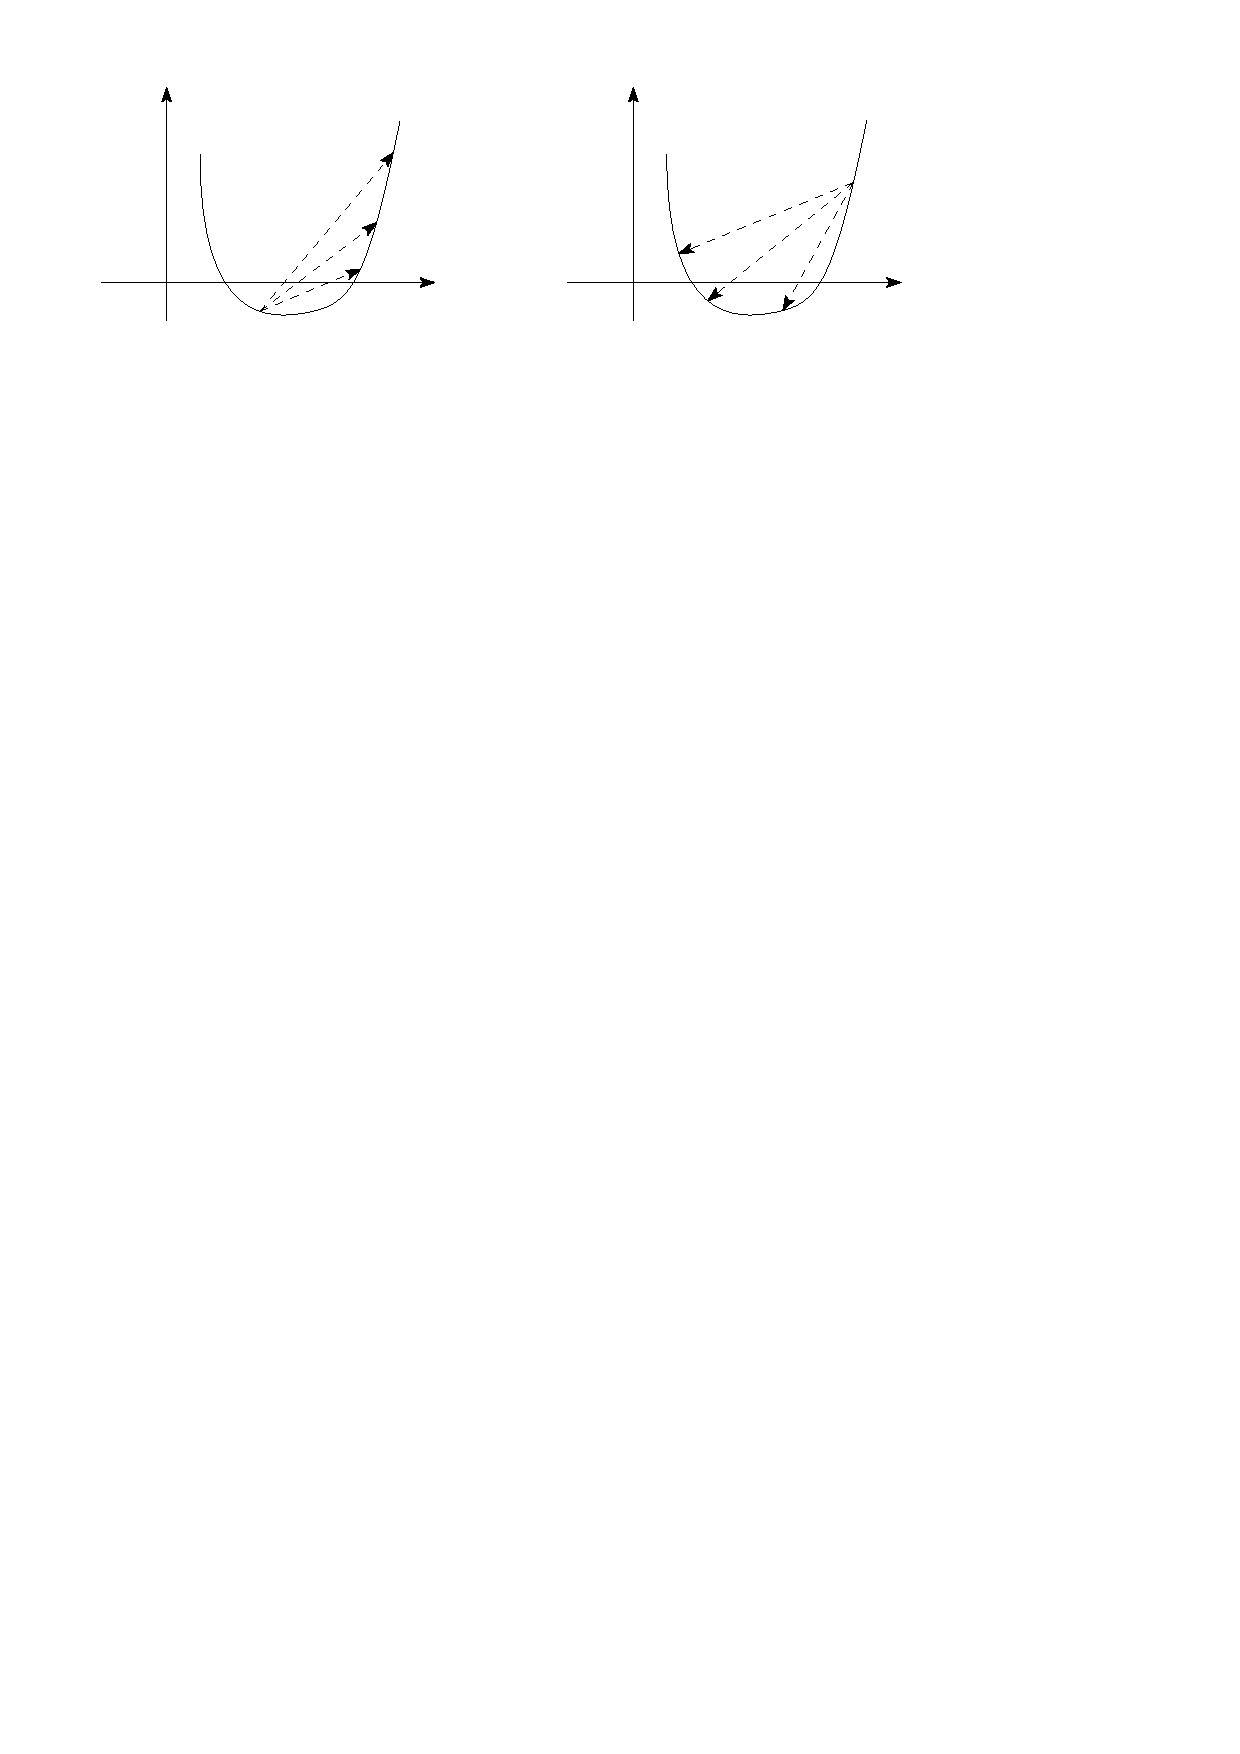
\includegraphics[scale = 0.8]{image/凸函数定理.pdf}
    \end{figure}
\end{theorem}
\begin{definition}[次梯度]
    非光滑图凸函数:存在$\boldsymbol{\xi}\in\mathbb{R}^n$使得
    \[
        f(\boldsymbol{y})\geqslant f(\boldsymbol{x})+\langle\boldsymbol{\xi},\boldsymbol{y}-\boldsymbol{x}\rangle,\quad\forall\boldsymbol{y}\in\mathbb{R}^n,
    \]
    $\boldsymbol{\xi}$称为凸函数$f(\boldsymbol{x})$在$x$点的次梯度。
\end{definition}
\begin{definition}[次微分]
    满足
    \[
        \partial f(\boldsymbol{x})=\{\boldsymbol{\xi}\in\mathbb{R}^n\mid f(\boldsymbol{y})\geqslant f(\boldsymbol{x})+\langle\boldsymbol{\xi},\boldsymbol{y}-\boldsymbol{x}\rangle,\forall\boldsymbol{y}\in\mathbb{R}^n\}.
    \]
    称
    \[
        h(\boldsymbol{y})\triangleq f(\boldsymbol{x})+\langle\boldsymbol{\xi},\boldsymbol{y}-\boldsymbol{x}\rangle 
    \]
    为函数$f(\boldsymbol{x})$在$\boldsymbol{x}$点的支撑超平面。
    \begin{figure}[htbp]
        \centering
        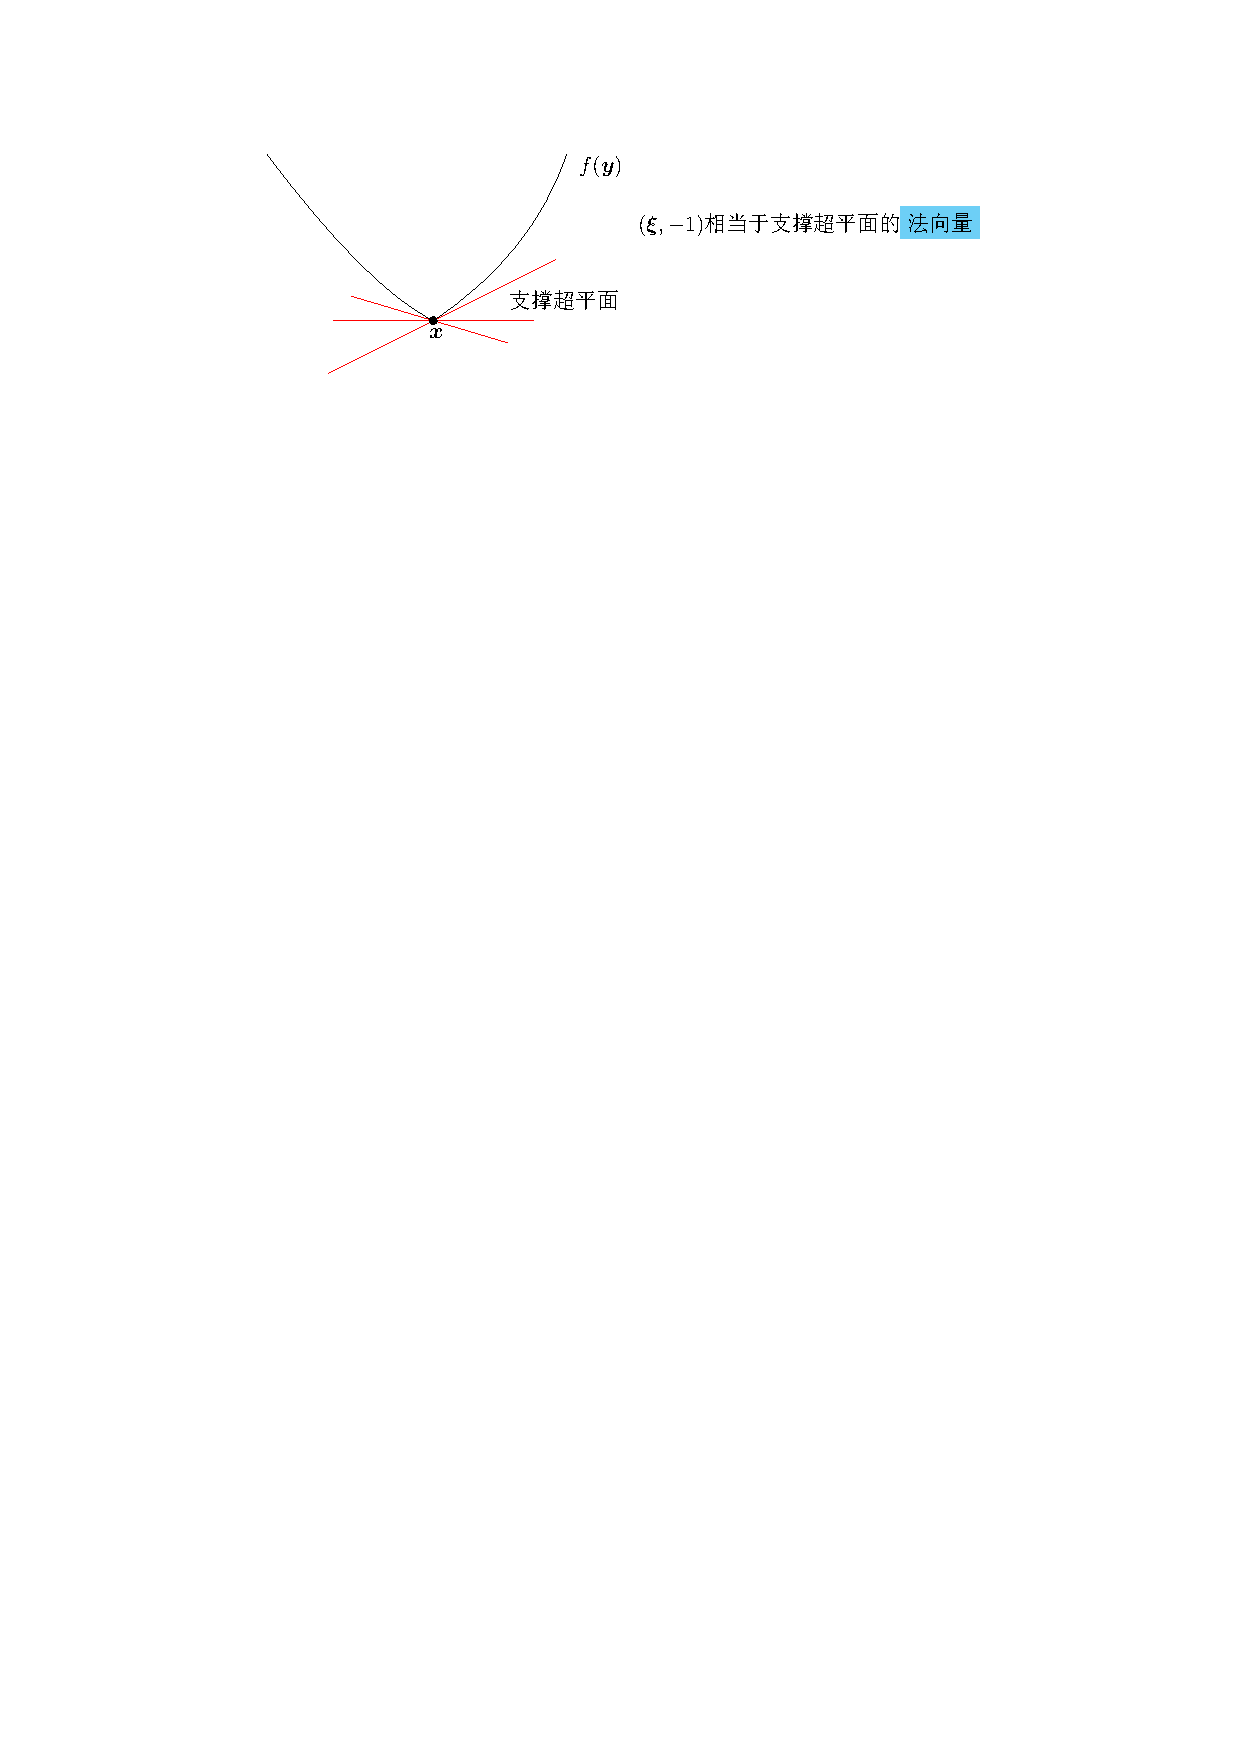
\includegraphics{image/支撑超平面.pdf}
    \end{figure}
\end{definition}
\begin{note}
    次梯度可能存在,可能不存在,也可能存在不唯一。
\end{note}
\begin{example}
    凸函数$f(x)=\begin{cases}-\sqrt{x},&x\geqslant0\\[2ex]\infty,&\text{else}\end{cases}$在零点没有次微分
    \begin{figure}[htbp]
        \centering
        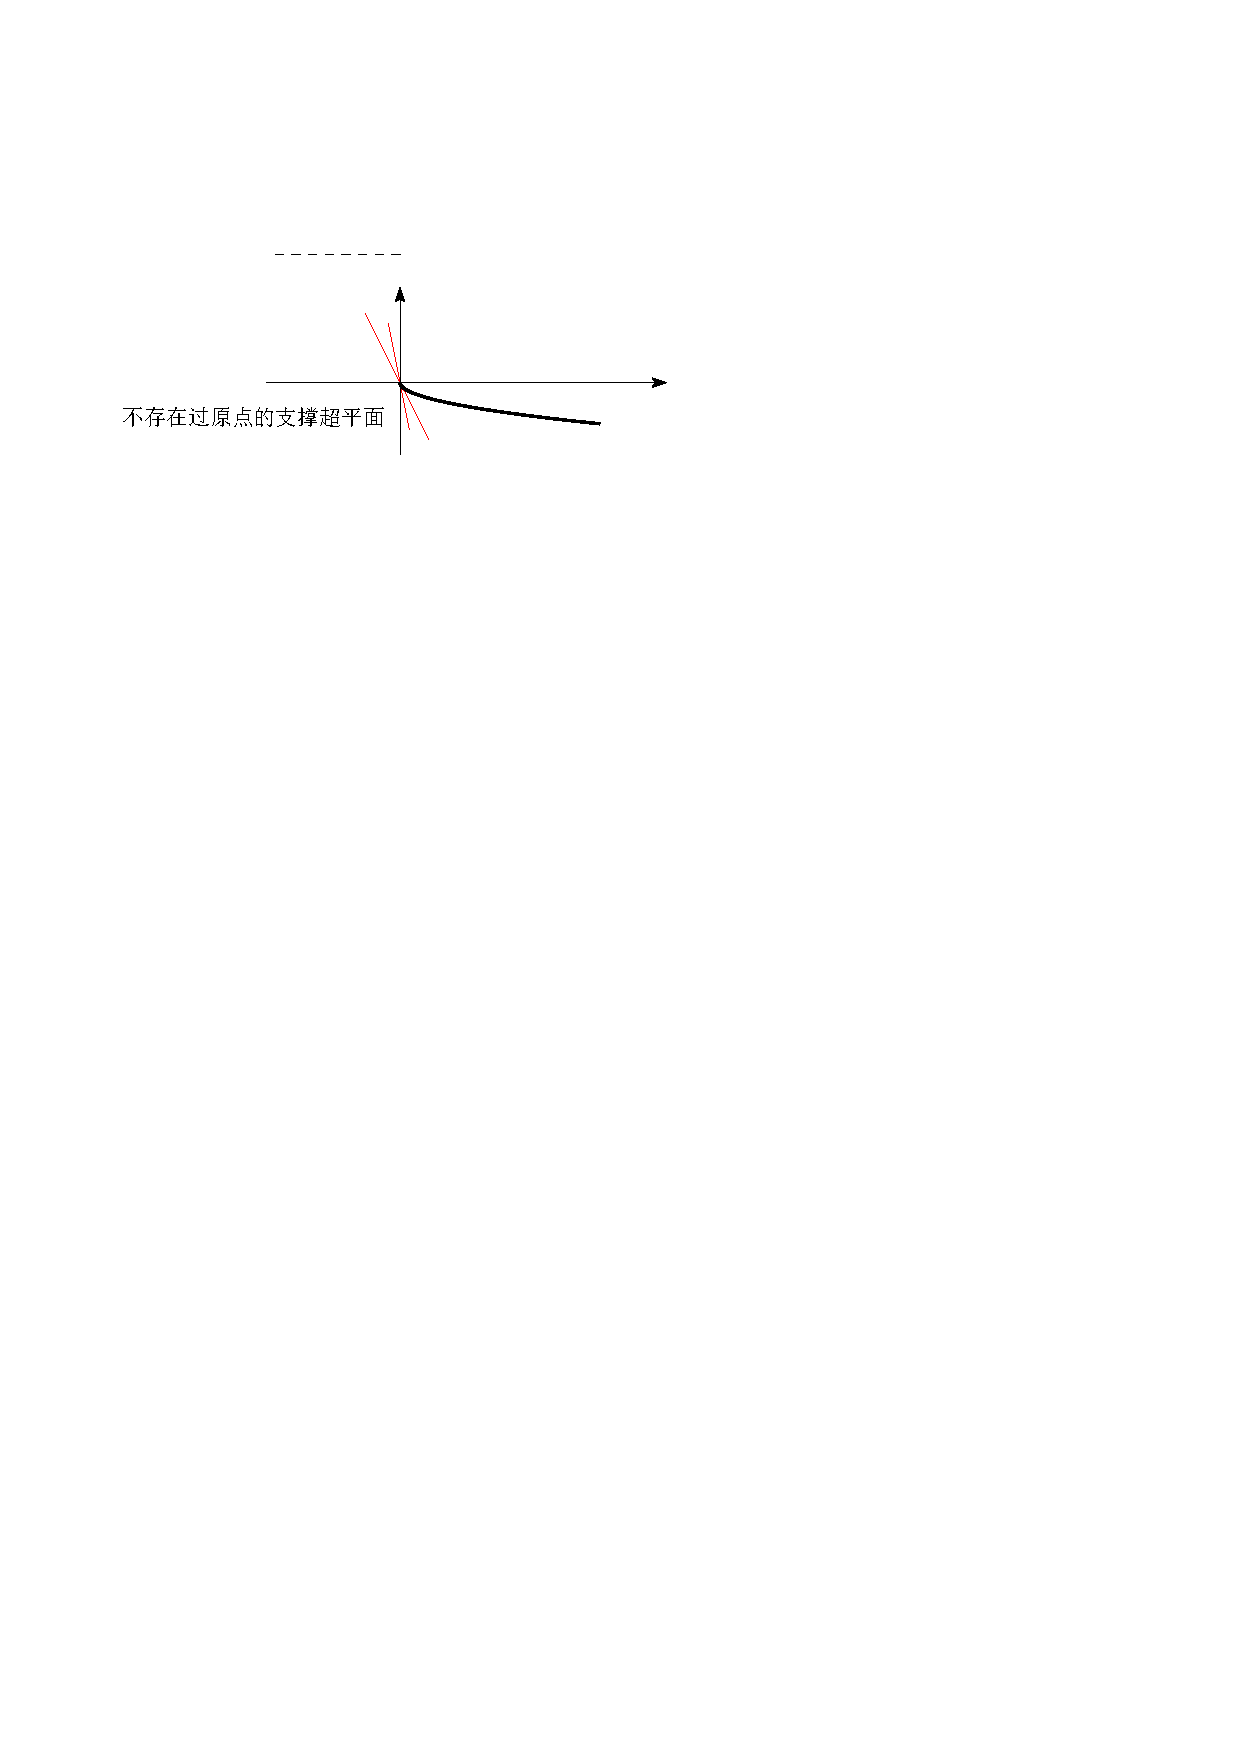
\includegraphics{image/支撑超平面example.pdf}
    \end{figure}
\end{example}
\begin{theorem}
    对凸函数$f:\mathbb{R}^n\to\mathbb{R}$,有
    \[
        \boldsymbol{\xi}\in\partial f(\boldsymbol{x})\Longleftrightarrow f'(\boldsymbol{x};\boldsymbol{d})\geqslant\boldsymbol{\xi}^\mathrm{T}\boldsymbol{d},\quad\forall \boldsymbol{d}\in\mathbb{R}^n.
    \]
\end{theorem}
\begin{theorem}
    $\boldsymbol{x}^*\in\mathbb{R}^n$为凸函数$f:\mathbb{R}^n\to\mathbb{R}$的最优值点当且仅当$\mathbf{0}\in\partial f(\boldsymbol{x})^*$
\end{theorem}
\begin{proof}
    \[
        \begin{array}{l}
            \mathbf{0}\in\partial f(\boldsymbol{x}^*)\\
            f(\boldsymbol{x})\geqslant f(\boldsymbol{x}^*)+\langle\boldsymbol{0},\boldsymbol{x}-\boldsymbol{x}^*\rangle,\quad\forall\boldsymbol{x}\in\mathbb{R}^n\\
            f(\boldsymbol{x})\geqslant f(\boldsymbol{x}^*),\quad\forall\boldsymbol{x}\in\mathbb{R}^n
        \end{array}
    \]
    证毕!
\end{proof}
\begin{note}
    次梯度是凸函数梯度的推广. 如果凸函数连续可微,则\colorbox{cyan!50}{梯度=次梯度}.
\end{note}
\begin{theorem}
    若凸函数$f:\mathbb{R}^n\to\mathbb{R}$在$\boldsymbol{x}$点可微,则
    \[
        \partial f(\boldsymbol{x})=\{\nabla f(\boldsymbol{x})\}
    \]
\end{theorem}
\begin{theorem}
    凸函数$f:\mathbb{R}^n\to\mathbb{R}$和其定义域内任一内点$\boldsymbol{x}$,$\partial f(x)$非空有界.
\end{theorem}
\begin{note}
    \colorbox{cyan!50}{凸函数一定次可微!可行域边界点除外。}
\end{note}
\begin{theorem}
    若$f:\mathbb{R}^n\to\mathbb{R}$在其定义域内部次可微, 则它为凸函数。
\end{theorem}
\begin{note}
    次梯度的推广:
    \begin{itemize}
        \item 非凸Lipschitz连续
        \[
            |f(\boldsymbol{x})-f(\boldsymbol{y})|\leqslant L\|\boldsymbol{x}-\boldsymbol{y}\|,\quad\forall\boldsymbol{x},\boldsymbol{y}\in\mathbb{R}^n
        \]
        \item 非凸局部Lipschitz连续
        \[
            |f(\boldsymbol{x})-f(\boldsymbol{y})|\leqslant L_{\boldsymbol{x}_0}\|\boldsymbol{x}-\boldsymbol{y}\|,\quad\forall\boldsymbol{x},\boldsymbol{y}\in N(\boldsymbol{x}_0,\delta)
        \]
    \end{itemize}
\end{note}
\subsubsection{临近点算子}
\begin{definition}[临近点算子]
    对函数$f:\mathbb{R}^n\to\mathbb{R}$,定义其在$\boldsymbol{x}\in\mathbb{R}^n$点的临近点算子
    \[
        \operatorname{prox}_f(\boldsymbol{x})=\arg\min_{\boldsymbol{y}\in\mathbb{R}^n}\Big\{f(\boldsymbol{y})+\frac{1}{2}\|\boldsymbol{y}-\boldsymbol{x}\|^2\Big\}
    \]
\end{definition}
\begin{note}
    临近点算子使子问题的性能得到加强, 如非凸函数变为凸函数,凸函数变为强凸函数, 便于在当前迭代点临近找到比该点更好的点.
\end{note}
\begin{definition}[临近点算子的扩展]
    \[
        \begin{aligned}
            \mathrm{prox}_{\frac{1}{L}f}(\boldsymbol{x})& =\underset{\boldsymbol{y}\in\mathbb{R}^{n}}{\arg\min}\Big\{f(\boldsymbol{y})+\frac{L}{2}\|\boldsymbol{y}-\boldsymbol{x}\|^{2}\Big\}  \\
            &=\underset{\boldsymbol{y}\in\mathbb{R}^{n}}{\arg\min}\Big\{\frac{1}{L}f\big(\boldsymbol{y}\big)+\frac{1}{2}\big\Vert\boldsymbol{y}-\boldsymbol{x}\big\Vert^{2}\Big\}
        \end{aligned}
    \]
    对于$f(\boldsymbol{x})+g(\boldsymbol{x})$,$f:\mathbb{R}^n\to\mathbb{R}$连续可微,$g:\mathbb{R}^n\to\mathbb{R}$连续
    \[
        \begin{array}{l}
            \arg\min\limits_{\boldsymbol{x}\in\mathbb{R}^{n}}\Big\{f(\boldsymbol{x}_{0})+\textcolor{red!50}{\underline{\nabla f(\boldsymbol{x}_{0})^{\mathrm{T}}(\boldsymbol{x}-\boldsymbol{x}_{0})+\dfrac{L}{2}\|\boldsymbol{x}-\boldsymbol{x}_{0}\|^{2}}}+g(\boldsymbol{x})\Big\}\\
            =\arg\operatorname*{min}\limits_{\boldsymbol{x}\in\mathbb{R}^{n}}\Big\{\dfrac{1}{L}g(\boldsymbol{x})+\textcolor{red!50}{\underline{\dfrac{1}{2}\|\boldsymbol{x}-\Big(\boldsymbol{x}_{0}-\dfrac{1}{L}\nabla f(\boldsymbol{x}_{0})\Big)\|^{2}}}\Big\}\\
            \stackrel{\triangle}{=}\mathrm{prox}_{\frac{1}{L}g}\bigl(\boldsymbol{x}_{0}-\dfrac{1}{L}\nabla f(\boldsymbol{x}_{0})\bigr)
        \end{array}
    \]
\end{definition}
\begin{example}
    求$f_2(x)=\begin{cases}0,&x\neq0\\[2ex]-\lambda,&x=0\end{cases}$的临近点算子$(\lambda>0)$。\Stars{5}{}

    \[
        \begin{aligned}
            \mathrm{prox}_{f_{2}}(x)& =\arg\min_{y\in\mathbb{R}}\left\{f_{2}(y)+\frac{1}{2}(y-x)^{2}\right\}  \\
            &=\arg\min_{y\in\mathbb{R}}\left\{\min_{y=0}\left\{-\lambda+\frac{x^{2}}{2}\right\},\min_{y\neq0}\left\{\frac{1}{2}(y-x)^{2}\right\}\right\} \\
            &=\arg\min_{y\in\mathbb{R}}\left\{-\lambda+\frac{x^{2}}{2},0\right\} \\
            &\left.=\left\{\begin{array}{ll}\{0\},&|x|<\sqrt{2\lambda}\\[2ex]\{x\},&|x|>\sqrt{2\lambda}\\[2ex]\{0,x\},&|x|=\sqrt{2\lambda}\end{array}\right.\right.
        \end{aligned}
    \]    
\end{example}
\begin{example}
    求$f_3(x)=\begin{cases}0,&x\neq0\\[2ex]\lambda,&x=0\end{cases}$的临近点算子$(\lambda>0)$。\Stars{5}{}

    解:
    \[
        \mathrm{prox}_{f_3}(x)=
            \left\{
                \begin{array}{cc}
                    \{x\}, & x\neq0\\
                    \emptyset, & x=0
                \end{array}
            \right.
    \]
\end{example}
\begin{definition}[下半连续]
    \[
        \lim_{\boldsymbol{x}\to\boldsymbol{x}_0}\inf f(\boldsymbol{x})\geqslant f(\boldsymbol{x}_0)
    \]
    \begin{figure}[htbp]
        \centering
        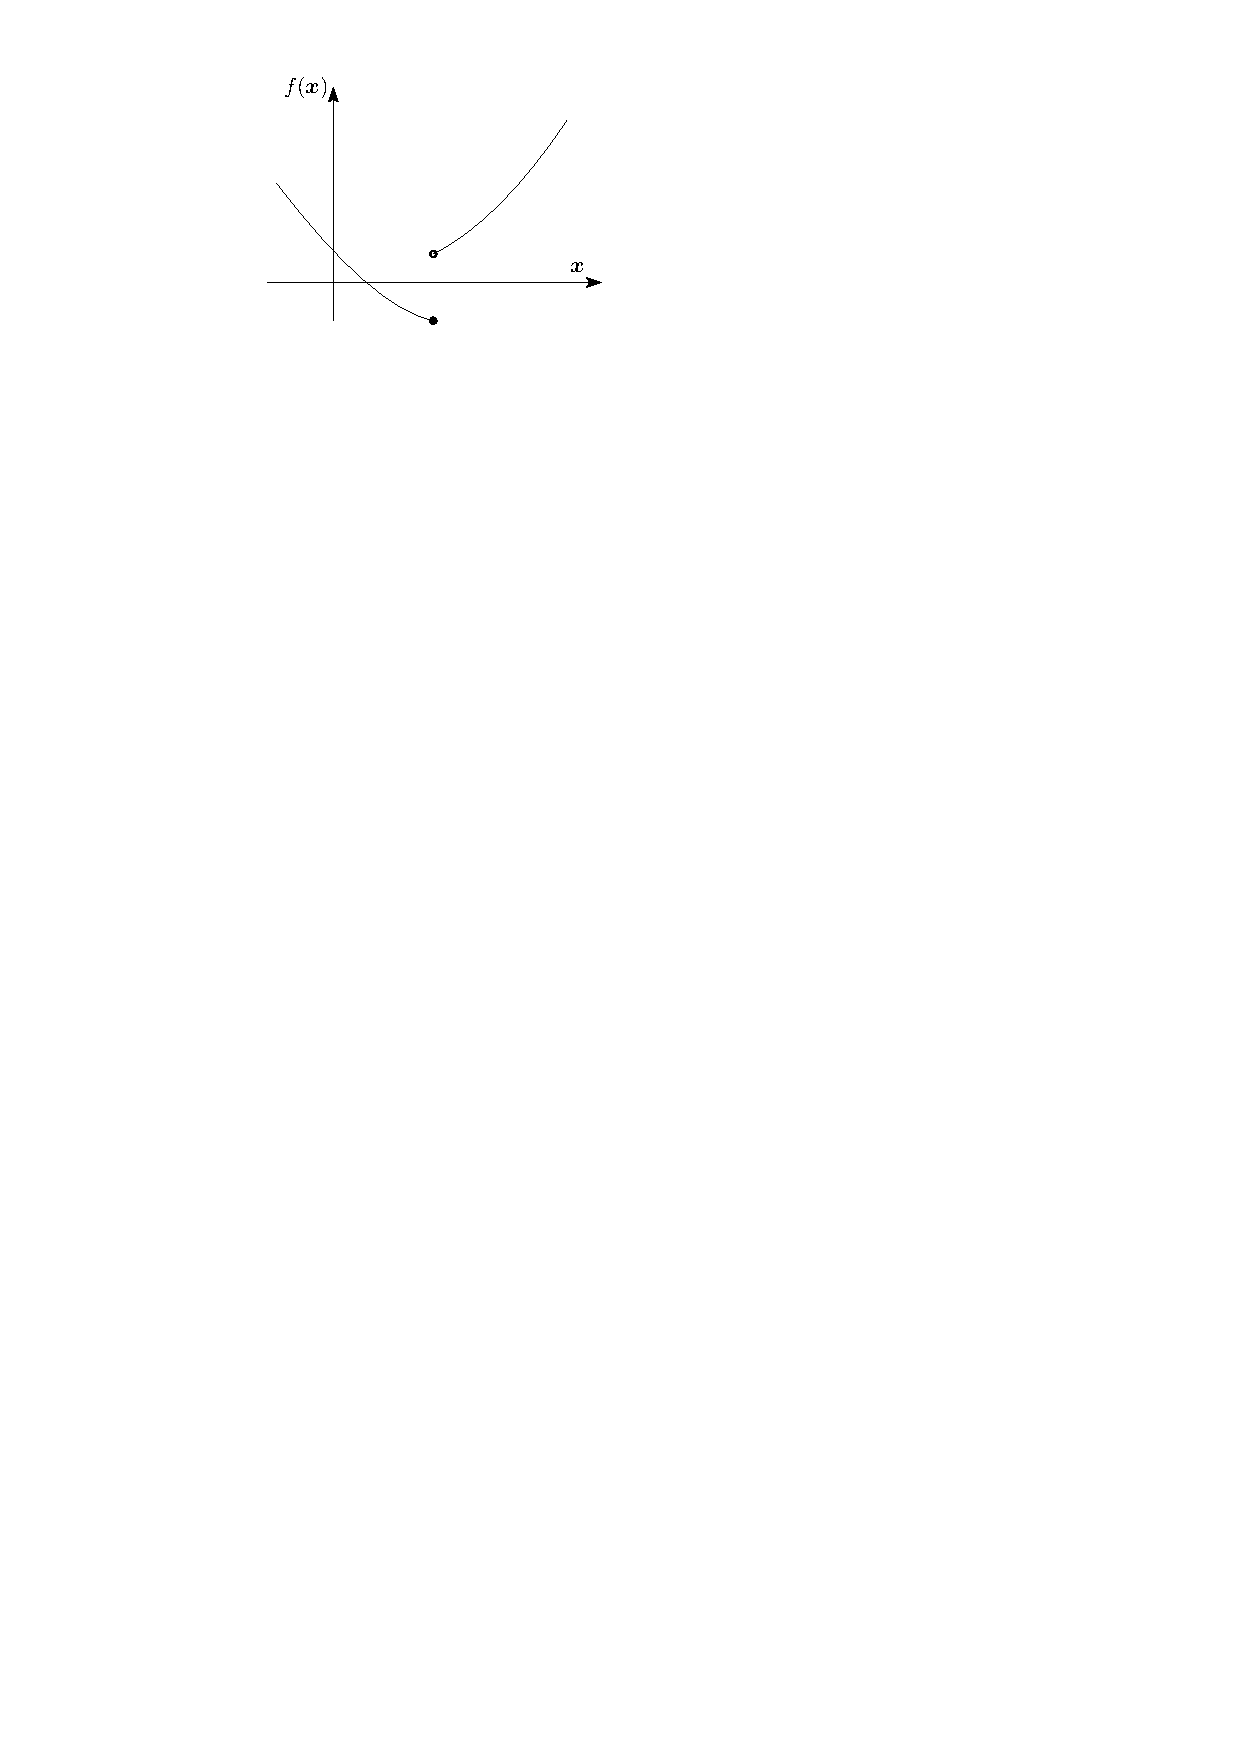
\includegraphics{image/下半连续.pdf}
    \end{figure}
\end{definition}
\begin{theorem}
    对下半连续的凸函数$f:\mathbb{R}^n\to\mathbb{R}$其临近点算子$\mathrm{prox}_{f}(\cdot)$为单一映射。
\end{theorem}
\begin{theorem}
    设凸函数$f:\mathbb{R}^n\to\mathbb{R}$下半连续.则对任意的$\boldsymbol{x},\boldsymbol{y}\in \mathbb{R}^{n}$ 
    \[
        \boldsymbol{y}=\mathrm{prox}_f(\boldsymbol{x})
    \]         
    \[
        \boldsymbol{x}-\boldsymbol{y}\in\partial f(\boldsymbol{y})
    \]
    \[
        \langle \boldsymbol{x}-\boldsymbol{y},\boldsymbol{z}-\boldsymbol{y}\rangle\leqslant f(\boldsymbol{z})-f(\boldsymbol{y}),\forall \boldsymbol{z}\in \mathbb{R}^{n}
    \]
\end{theorem}
\begin{proof}
    由临近点算子的定义,对任意的$\boldsymbol{x},\boldsymbol{y}\in \mathbb{R}^n$
    \[
        \boldsymbol{y}=\mathrm{prox}_{f}(\boldsymbol{x})\Longleftrightarrow \boldsymbol{y}=\arg\min_{\boldsymbol{z}\in\mathbb{R}^{n}}\{f(\boldsymbol{z})+\frac{1}{2}\|\boldsymbol{z}-\boldsymbol{x}\|^{2}\}.
    \]
    后面等价于$\boldsymbol{0}\in\partial f(\boldsymbol{y})+\boldsymbol{y}-\boldsymbol{x}.$
    由次梯度的定义$\boldsymbol{x}-\boldsymbol{y}\in\partial f(\boldsymbol{y})$等价于,
    \[
        \langle \boldsymbol{x}-\boldsymbol{y},\boldsymbol{z}-\boldsymbol{y}\rangle\leqslant f(\boldsymbol{z})-f(\boldsymbol{y}),\forall \boldsymbol{z}\in \mathbb{R}^{n}
    \]
    证毕!
\end{proof}
\begin{theorem}
   设$f$为下半连续的凸函数. 则对任意$\boldsymbol{x},\boldsymbol{y}\in \mathbb{R}^n$
   \[
        \langle\boldsymbol{x}-\boldsymbol{y},\mathrm{prox}_f(\boldsymbol{x})-\mathrm{prox}_f(\boldsymbol{y})\rangle\geqslant\|\mathrm{prox}_f(\boldsymbol{x})-\mathrm{prox}_f(\boldsymbol{y})\|^2
   \]
   \[
        \|\mathrm{prox}_f(\boldsymbol{x})-\mathrm{prox}_f(\boldsymbol{y})\|\leqslant\|\boldsymbol{x}-\boldsymbol{y}\|.
   \]
\end{theorem}
\subsubsection{和式优化最优性条件}
为充分利用函数的解析性质,将目标函数中的项根据其解析性质分开,可得如下和式优化问题
\[
    \min_{\boldsymbol{x}\in\mathbb{R}^n}f(\boldsymbol{x})+g(\boldsymbol{x})
\]
用梯度和次梯度建立优化问题的最优性条件
\begin{theorem}
    $\boldsymbol{x}^*\in\mathbb{R}^n$为优化问题$\operatorname*{min}_{\boldsymbol{x}\in\mathbb{R}^n}f(\boldsymbol{x})+g(\boldsymbol{x})$的最优解,则$-\nabla f(\boldsymbol{x}^*)\in\partial g(\boldsymbol{x}^*)$
\end{theorem}
% \begin{proof}
%     任取$\boldsymbol{x}\mathbb{}$
% \end{proof}
\subsection{线性化临近点方法}
用梯度和函数值建立优化问题的最优性条件
\[
    \min f(\boldsymbol{x})+g(\boldsymbol{x})
\]
其中$\Omega\subset\mathbb{R}^n$,$f:\mathbb{R}^n\to\mathbb{R}$连续可微的凸函数,$g:\mathbb R^n\to\mathbb R$凸函数
\begin{theorem}
    为上述优化问题的最优解当且仅当
    \[
        g(\boldsymbol{x})-g(\boldsymbol{x}^*)+\nabla f(\boldsymbol{x}^*)^\mathrm{T}(\boldsymbol{x}-\boldsymbol{x}^*)\geqslant 0,\quad\forall\boldsymbol{x}\in\mathbb{R}^n
    \]
\end{theorem}
\begin{note}
    临近点算法
    \[
        \boldsymbol{x}_{k+1}=\arg\min_{\boldsymbol{x}\epsilon\mathbb{R}^{n}}\left\{f(\boldsymbol{x})+\frac{L}{2}\|\boldsymbol{x}-\boldsymbol{x}_{k}\|^{2}\right\}
    \]
\end{note}
\begin{note}
    算法收敛性
    \[
        \boldsymbol{x}_{k+1}=\arg\min_{\boldsymbol{x}\in\mathbb{R}^n}\left\{f(\boldsymbol{x})+\frac{L}{2}\|\boldsymbol{x}-\boldsymbol{x}_k\|^2\right\}
    \]
    由
    \begin{figure}[H]
        \centering
        
\includegraphics{image/临近点算子收敛性.pdf}
    \end{figure}
    得
    \[
        f(\boldsymbol{x})-f(\boldsymbol{x}_{k+1})+L(\boldsymbol{x}_{k+1}-\boldsymbol{x}_k)^\mathrm{T}(\boldsymbol{x}-\boldsymbol{x}_{k+1})\geqslant0,\quad\forall\boldsymbol{x}\in\mathbb{R}^n
    \]
    令$\boldsymbol{x} = \boldsymbol{x}_{k}$
    \[
        f(\boldsymbol{x}_k)-f(\boldsymbol{x}_{k+1})\geqslant L\|\boldsymbol{x}_k-\boldsymbol{x}_{k+1}\|^2.
    \]
    \[
        f(\boldsymbol{x}_0)-\lim_{k\to\infty}f(\boldsymbol{x}_k)\geqslant L\sum_{k=0}^\infty\|\boldsymbol{x}_k-\boldsymbol{x}_{k+1}\|^2\longrightarrow\lim_{k\to\infty}\|\boldsymbol{x}_k-\boldsymbol{x}_{k+1}\|=0.
    \]
    算法产生的函数值序列$\left\{ f(\boldsymbol{x}) \right\}$单调不增.如果目标函数$f(\boldsymbol{x})$在$\mathbb{R}^n$上有下界, 则数列$\left\{ f(\boldsymbol{x}) \right\}$收敛. 
\end{note}
\begin{theorem}
    $f:\mathbb{R}^n\to\mathbb{R}$下半连续的凸函数,有下界;临近点算法$\boldsymbol{x}_{k+1}=\mathrm{prox}_{\frac1Lf}(\boldsymbol{x}_k)$产生迭代点列的任一聚点为凸优化问题$\min\limits_{\boldsymbol{x}\in\mathbb{R}^{n}}f(\boldsymbol{x})$的最优值点.

\end{theorem}
\subsection{交替极小化方法}
\[
    \min_{\boldsymbol{x}_1\in\mathbb{R}^{n_1},\boldsymbol{x}_2\in\mathbb{R}^{n_2},\cdots,\boldsymbol{x}_s\in\mathbb{R}^{n_s}}\Psi(\boldsymbol{x}_1,\boldsymbol{x}_2,\cdots,\boldsymbol{x}_s)
\]
以循环方式交替对$s$个块变量求最小。
对迭代点$\boldsymbol{x}^k=(\boldsymbol{x}_1^k,\boldsymbol{x}_2^k,\cdotp\cdotp\cdotp,\boldsymbol{x}_s^k), $分别基于块变量依次对$\boldsymbol{x}_1,\boldsymbol{x}_2,\cdots,\boldsymbol{x}_s$求极小, 得到新的迭代点
\[
    \begin{aligned}
        &\boldsymbol{x}^{k,1}=(\boldsymbol{x}_{1}^{k+1},\boldsymbol{x}_{2}^{k},\cdots,\boldsymbol{x}_{s}^{k}),\\
        &\boldsymbol{x}^{k,2}=(\boldsymbol{x}_{1}^{k+1},\boldsymbol{x}_{2}^{k+1},\boldsymbol{x}_{3}^{k},\cdots,\boldsymbol{x}_{s}^{k}),\\
        &\boldsymbol{x}^{k,i}=(\boldsymbol{x}_{1}^{k+1},\boldsymbol{x}_{2}^{k+1},\cdots,\boldsymbol{x}_{i}^{k+1},\boldsymbol{x}_{i+1}^{k},\cdots,\boldsymbol{x}_{s}^{k}),\\
        &\boldsymbol{x}^{k,s}=\boldsymbol{x}^{k+1}=(\boldsymbol{x}_{1}^{k+1},\boldsymbol{x}_{2}^{k+1},\cdots,\boldsymbol{x}_{s}^{k+1}).
    \end{aligned}
\]

\begin{theorem}
    设目标函数$\Psi:\mathbb{R}^{n}\to\mathbb{R}$连续可微,目标函数水平集有界且对任意的$\boldsymbol{x}\in\mathbb{R}^n$和$i\in\left\{ 1,2,\cdots,s \right\}$
    \[
        \operatorname*{min}_{\boldsymbol{y}\in\mathbb{R}^{n_{i}}}\Psi(\boldsymbol{x}_{1},\boldsymbol{x}_{2},\cdots,\boldsymbol{x}_{i-1},\boldsymbol{y},\boldsymbol{x}_{i+1},\cdots,\boldsymbol{x}_{s})
    \]
    有唯一最优解. 则算法产生迭代点列的任一聚点为优化问题的稳定点.
\end{theorem}
\begin{example}
    反例:连续不可微.$\min\Psi(x_1,x_2)=|3x_1+4x_2|+|x_1-2x_2|$\Stars{5}{}
    \begin{solution}
        连续凸函数, 水平集有界, 且对任一分量有唯一最优解.对任意$\alpha>0$,
        \[
            \Psi(-4\alpha,t)=|4t-12\alpha|+|2t+4\alpha|=
            \begin{cases}-6t+8\alpha,&\quad t<-2\alpha,\\
                -2t+16\alpha,&\quad-2\alpha\leqslant t\leqslant 3\alpha\\
                6t-8\alpha,&\quad t>3\alpha,
            \end{cases}
        \]
        \[
            \Psi(t,3\alpha)=|3t+12\alpha|+|t-6\alpha|=
            \begin{cases}
                -4t-6\alpha,&\quad t<-4\alpha,\\
                2t+18\alpha,&\quad-4\alpha\leqslant t\leqslant6\alpha,\\
                4t+6\alpha,&\quad t>6\alpha,
            \end{cases}
        \]
        对任意$\alpha\leqslant 0$
        \[
            \begin{array}{l}
                -4\alpha=\arg\min_{x_{1}\in \mathbb{R}}\Psi(x_{1},3\alpha),\\3\alpha=\arg\min_{x_{2}\in \mathbb{R}}\Psi(-4\alpha,x_{2})
            \end{array}
        \]
        交替极小化方法
        \[
            \min\Psi(x_{1},x_{2})=|3x_{1}+4x_{2}|+|x_{1}-2x_{2}|
        \]
        若$x_1$非零,则在首次迭代后, 算法滞留在\colorbox{cyan!50}{$(-4\alpha,3\alpha)$点(聚点)}。\newline$\boldsymbol{x} = \boldsymbol{0}$为函数的唯一最小值点,$(-4\alpha,3\alpha)$既不是该函数的最小值点, 也不是其稳定点。
    \end{solution}    
\end{example}
\begin{definition}[坐标轮换最小值点]
    若$\boldsymbol{x}^*\in\mathbb{R}^n$满足
    \[
        \Psi(\boldsymbol{x}^*)\leqslant\Psi(\boldsymbol{x}_1^*,\cdotp\cdotp\cdotp,\boldsymbol{x}_{i-1}^*,\boldsymbol{x}_i,\boldsymbol{x}_{i+1}^*,\cdotp\cdotp\cdotp,\boldsymbol{x}_s^*),
    \]
    $\forall i=1,2,\cdots,s,\boldsymbol{x}_i\in\mathbb{R}^{n_i},$则称$\boldsymbol{x}^*$为函数$\Psi(\boldsymbol{x})$的坐标轮换最小值点。
\end{definition}
\begin{theorem}
    设优化问题
    \[
        \min_{\boldsymbol{x}_1\in \mathbb{R}^{n_1},\boldsymbol{x}_2\in\mathbb{R}^{n_2},\cdotp\cdotp\cdotp,\boldsymbol{x}_s\in\mathbb{R}^{n_s}}\Psi(\boldsymbol{x}_1,\boldsymbol{x}_2,\cdotp\cdotp\cdotp,\boldsymbol{x}_s)  
    \]
    目标函数下半连续,水平集有界,子问题
    \[
        \min_{\boldsymbol{y}\in\mathbb{R}^ni}\Psi(\boldsymbol{x}_1,\cdots,\boldsymbol{x}_{i-1},\boldsymbol{y},\boldsymbol{x}_{i+1},\cdots,\boldsymbol{x}_s)
    \]
    有唯一最优解。 则迭代点列的任一聚点为坐标轮换最小值点.
\end{theorem}
\begin{note}
    连续不可微函数的坐标轮换极小值点未必是其最小值点或稳定点.那么,在什么情况下是呢?
\end{note}
\begin{theorem}
    对优化问题
    \[
        \min_{\boldsymbol{x}\in\mathbb{R}^n}\Psi(\boldsymbol{x})=f(\boldsymbol{x})+g(\boldsymbol{x})
    \]
    $f:\mathbb{R}^n\to\mathbb{R}$连续可微,              
    $g(\boldsymbol{x})=\sum_{i=1}^sg_i(\boldsymbol{x}_i),g_{i}:\mathbb{R}^{n_{i}}\to\mathbb{R}$连续凸函数。

    \begin{center}
        坐标轮换极小值$\Longleftrightarrow$稳定点
    \end{center}

    \colorbox{red!50}{对分块和式优化问题,若子问题最优解不唯一,算法收敛性不能保证。}
\end{theorem}
\begin{example}
    反例:子问题最优解不唯一\Stars{5}{}
    \begin{solution}
        \[
            \begin{aligned}
                f(x,y,z)=&-xy-yz-zx+[x-1]_{+}^{2}+[-x-1]_{+}^{2}+[y-1]_{+}^{2}\\
                &+[-y-1]_{+}^{2}+[z-1]_{+}^{2}+[-z-1]_{+}^{2}.
            \end{aligned}
        \]
        依次两两固定$y,z,x$\colorbox{cyan!50}{(注:$[x]_{+} = \frac{x+|x|}{2}$)}
        \[
            \begin{aligned}
                f(x;y,z) &= -x(y+z)+\left( \dfrac{(x-1)+|x-1|}{2} \right)^2+\left( \dfrac{-(x+1)+|x+1|}{2} \right)^2 + a \\
                &=\begin{cases}
                    -x(y+z)+(x+1)^2+a & x<-1 \\
                    -x(y+z)+0+a & -1<x<1 \\
                    -x(y+z)+ (x-1)^2+a & x>1
                \end{cases}
            \end{aligned}
        \]
        \[
            f'_x(x;y,z) =\begin{cases}
                2(x+1)-(y+z) & x<-1 \\
                -(y+z)& -1<x<1 \\
                2(x-1)-(y+z) & x>1
            \end{cases}
        \]
        根据$f'_x(x;y,z) = 0$,得到
        \newline
        $x<-1$时,$x = -1+\frac{y+z}{2}$,(\colorbox{cyan!50}{$y+z<0$时取到})
        \newline
        $x>1$时,$x = 1+\frac{y+z}{2}$,(\colorbox{cyan!50}{$y+z>0$时取到})
        故而,有
        \[
            \arg\min_xf(x,y,z)=
            \begin{cases}
                \operatorname{sgn}(y+z)\big(1+\frac{1}{2}|y+z|\big),&y+z\neq0,\\
                [-1,1],&y+z=0.
            \end{cases}
        \]
        \[
            \arg\min\limits_{y}f(x,y,z)=
            \begin{cases}
                \operatorname{sgn}(x+z)\big(1+\frac{1}{2}|x+z|\big),&x+z\neq0,\\
                [-1,1],&x+z=0,
            \end{cases}
        \]
        \[
            \arg\min_zf(x,y,z)=
            \begin{cases}
                \operatorname{sgn}(x+y)(1+\frac{1}{2}|x+y|),&x+y\neq0,\\
                [-1,1],&x+y=0.
            \end{cases}    
        \]
    \end{solution}
\end{example}
\subsubsection{和式凸优化交替极小化方法}
\[
    \min_{x\in\mathbb{R}^n}\Psi(\boldsymbol{x})=f(\boldsymbol{x})+g(\boldsymbol{x})
\]
$f:\mathbb{R}^n\to\mathbb{R}$ 连续可微的凸函数
\newline
$g(\boldsymbol{x})=\sum_{i=1}^{s}g_{i}(\boldsymbol{x}_{i}),\quad g_{i}:\mathbb{R}^{n_{i}}\to\mathbb{R}$连续凸函数

对该优化问题,无需子问题最优解唯一, 就能建立算法的全局收敛性. 
\begin{theorem}
    对上述优化问题,若目标函数水平集有界, 则交替极小化方法产生迭代点列的任一聚点为问题的最优解.
\end{theorem}
\subsubsection{二分块交替极小化方法}
\[
    \min_{\boldsymbol{x}_1\in\mathbb{R}^{n_1},\boldsymbol{x}_2\in\mathbb{R}^{n_2}}\{\Psi(\boldsymbol{x}_1,\boldsymbol{x}_2)=f(\boldsymbol{x}_1,\boldsymbol{x}_2)+g_1(\boldsymbol{x}_1)+g_2(\boldsymbol{x}_2)\}
\]
$f:\mathbb{R}^n\to\mathbb{R}$ 连续可微的凸函数
\newline
$\nabla_if(x)$ Lipschitz连续,常数为 $L_i,i=1,2$ 
\newline
$g_i:\mathbb{R}^{n_i}\to\mathbb{R}$ 下半连续的凸函数

\begin{note}
    二分块交替极小化算法
    \begin{itemize}
        \item 初始步:取$\boldsymbol{x}_1^0\in\mathbb{R}^{n_1}$,计算
        \[
            \boldsymbol{x}_2^0=\arg\min_{\boldsymbol{x}_2}f(\boldsymbol{x}_1^0,\boldsymbol{x}_2)+g_2(\boldsymbol{x}_2)    
        \]
        \item 选代步:依次计算
        \[
            \begin{array}{l}
                \boldsymbol{x}_{1}^{k+1}=\arg\min_{\boldsymbol{x}_{1}}f(\boldsymbol{x}_{1},\boldsymbol{x}_{2}^{k})+g_{1}(\boldsymbol{x}_{1}),\\
                \boldsymbol{x}_{2}^{k+1}=\arg\min_{\boldsymbol{x}_{2}}f(\boldsymbol{x}_{1}^{k+1},\boldsymbol{x}_{2})+g_{2}(\boldsymbol{x}_{2}).
            \end{array}
        \]
    \end{itemize}
\end{note}
   
\subsection{凸分析基础II}
\subsubsection{凸集与凸集分离定理}
\begin{definition}[锥]
    $\mathcal{K}\subset\mathbb{R}^n$对任意的$\boldsymbol{x}\in \mathcal{K}$和$\lambda\leqslant 0$,都有$\lambda\boldsymbol{x}\in \mathcal{K}$。

    \colorbox{red!50}{并不是所有的锥都是凸的}
\end{definition}
\begin{definition}[极锥]
    与原锥对立的锥。
    \[
        \mathcal{K}^{\circ}=\{\boldsymbol{y}\in\mathbb{R}^{n}\mid\langle \boldsymbol{x},\boldsymbol{y}\rangle\leqslant0,\forall \boldsymbol{x}\in\mathcal{K}\}.
    \]
    \colorbox{red!50}{子空间的极锥为其正交补空间!}
\end{definition}
\begin{definition}[闭凸集的切锥]
    $\Omega$为$\mathbb{R}^n$中的非空闭凸集,$\boldsymbol{x}
    \in \Omega$。
    \[
        \mathcal{T}_{\Omega}(\boldsymbol{x})=\{\boldsymbol{d}\in\mathbb{R}^{n}\mid\text{存在 }\boldsymbol{d}_{k}\rightarrow\boldsymbol{d},t_{k}\downarrow0,\text{使得}\boldsymbol{x}+t_{k}\boldsymbol{d}_{k}\in\Omega\}
    \]
    定义为凸集$\Omega$在该点的切锥.
    \[
        \text{切锥 }\mathcal{T}_\Omega(\boldsymbol{x})\text{ 的极锥 }\mathcal{T}_\Omega^\circ(\boldsymbol{x})\text{ 称为集合}\Omega\text{在 }\boldsymbol{x}\text{ 点的法锥或正则锥},\text{记为}\mathcal{N}_\Omega(\boldsymbol{x})
    \]
\end{definition}
\begin{definition}[有限生成锥]
    锥中任一元素都可以表示有限个元素的非负组合, 即
    \[
        \mathcal{K}=\Big\{\sum_{i=1}^{m}\mu_{i}\boldsymbol{b}_{i}\big|\mu_{i}\geqslant0,i=1,2,\cdots,m\Big\},
    \]
    $\boldsymbol{b}_{1},\boldsymbol{b}_{2},\cdots,\boldsymbol{b}_{m}$称为生成元。
    
    \colorbox{red!50}{有限生成锥是凸锥,它等价于多面锥。}
\end{definition}
\begin{definition}[多面锥]
    可以表示成如下形式的锥    
    \[
        \mathcal{K}=\{\boldsymbol{x}\in\mathbb{R}^n\mid\boldsymbol{Ax}\geqslant\boldsymbol{0}\}
    \]
\end{definition}
\begin{definition}[凸组合]
    设$\boldsymbol{x}_1,\boldsymbol{x}_2,\cdots,\boldsymbol{x}_m\in\mathbb{R}^n,\lambda_i\geqslant0,i=1,2,\cdots,m$满足$\lambda_{1}+\lambda_{2}+\cdots+\lambda_{m}=1$,称
    \[
        \lambda_1\boldsymbol{x}_1+\lambda_2\boldsymbol{x}_2+\cdots+\lambda_m\boldsymbol{x}_m
    \]
    为$\boldsymbol{x}_1,\boldsymbol{x}_2,\cdots,\boldsymbol{x}_m$的一个凸组合.
\end{definition}
\begin{definition}[凸包]
    $\boldsymbol{x}_1,\boldsymbol{x}_2,\cdots,\boldsymbol{x}_m$的所有凸组合构成的集合称为由其生成的凸包.
\end{definition}
\begin{definition}[多面胞]
    含有限个顶点的闭凸集,又称多面胞.
    \[
        \mathcal{S}=\{\boldsymbol{x}\in\mathbb{R}^{n}\mid\boldsymbol{A}\boldsymbol{x}\geqslant\boldsymbol{b}\}
    \]
    有界的凸多面体就是多面胞
\end{definition}
\begin{definition}[回收方向]
    $\boldsymbol{d}$满足
    \[
        \forall\boldsymbol{x}\in\mathcal{S},\alpha\geqslant0\Longrightarrow x+\alpha\boldsymbol{d}\in\mathcal{S}
    \]
\end{definition}
\begin{theorem}
    若多面体$\mathcal{S}=\{\boldsymbol{x}\mid\boldsymbol{A}\boldsymbol{x}\geqslant\boldsymbol{b}\}$无界, 则存在多面胞$\mathcal{P}$和多面锥$\mathcal{K}$使得
    \[
        \mathcal{S}=\mathcal{P}+\mathcal{K}.
    \]
    \[
        \mathcal{P} = \left\{ \boldsymbol{x}|\boldsymbol{Ax} = b \right\}
    \]
    \[
        \mathcal{K} = \left\{ \boldsymbol{x}|\boldsymbol{Ax} \geqslant \boldsymbol{0} \right\}
    \]
\end{theorem}
\begin{definition}[仿射集]
    $\boldsymbol{x}_1,\boldsymbol{x}_2,\cdots,\boldsymbol{x}_m\in\mathbb{R}^n,\lambda_i\in \mathbb{R},i=1,2,\cdots,m$满足$\lambda_{1}+\lambda_{2}+\cdots+\lambda_{m}=1$,称
    \[
        \lambda_1\boldsymbol{x}_1+\lambda_2\boldsymbol{x}_2+\cdots+\lambda_m\boldsymbol{x}_m
    \]
    为$\boldsymbol{x}_1,\boldsymbol{x}_2,\cdots,\boldsymbol{x}_m$的一个仿射组合.
\end{definition}
\begin{definition}[内点]
    存在该点的邻域$N(\boldsymbol{x},\delta)$,使得$N(\boldsymbol{x},\delta)\subseteq \mathcal{S}$
\end{definition}
\begin{definition}[相对内点]
    存在该点的邻域$N(\boldsymbol{x},\delta)$,使得$N(\boldsymbol{x},\delta)\cap \operatorname{Aff}(\mathcal{S})\subset \mathcal{S}$。
    即该点在仿射子空间$\operatorname{Aff(\mathcal{S})}$中是集合的内点
\end{definition}
\begin{theorem}[凸集分离定理]
    设$\mathcal{S}\subset \mathbb{R}^n$是非空闭凸集,$\boldsymbol{y}\notin \mathcal{S}$。则存在非零向量$\boldsymbol{p}$和常数$\alpha$使得
    \[
        \boldsymbol{p}^{\mathrm{T}}\boldsymbol{y}>\alpha,\boldsymbol{p}^{\mathrm{T}}\boldsymbol{x}\leqslant\alpha,\forall \boldsymbol{x}\in\mathcal{S}
    \]

    直观意义:若点$\boldsymbol{y}$不属于闭凸集$\mathcal{S}$,则存在超平面
    \[
        H=\{\boldsymbol{x}\mid\boldsymbol{p}^{\mathrm{T}}\boldsymbol{x}=\alpha\}
    \]
    将该点与闭凸集严格分离.
    \colorbox{red!50}{这种分离不是唯一的!}
\end{theorem}
\begin{theorem}[Farkas引理]
    向量$\boldsymbol{b}$可以表示为向量组$\boldsymbol{a}_1,\boldsymbol{a}_2,\cdots,\boldsymbol{a}_m$的非负线性组合的充要条件是对任意满足$\boldsymbol{a}_{i}^{\mathrm{T}}\geqslant 0$的$\boldsymbol{x}$,都有
    $\boldsymbol{b}^{\mathrm{T}}\boldsymbol{x}\geqslant 0$
\end{theorem}
\begin{theorem}[Farkas引理']
    对于$\boldsymbol{A}\in\mathbb{R}^{n\times m},\boldsymbol{b}\in\mathbb{R}^{n}$下述两系统恰有一个解
    \begin{enumerate}
        \item $\boldsymbol{A}^\mathrm{T}\boldsymbol{x}\geqslant\boldsymbol{0},\boldsymbol{b}^\mathrm{T}\boldsymbol{x}<0;$
        \item $\boldsymbol{Ay}=\boldsymbol{b},\boldsymbol{y}\geqslant0.$
    \end{enumerate}
\end{theorem}


%\printbibliography[heading=bibintoc, title=\ebibname]

\end{document}
